Dans le chapitre précédent, nous avons décrit l'instrument NIKA2, installé au télescope de 30 mètres de l'IRAM, et ses performances.
Nous avons vu en quoi ses performances étaient parfaitement adaptées aux observations de l'effet SZ en direction d'amas de galaxies, et expliqué comment sont réalisées les observations avec NIKA2.

Dans ce chapitre, nous présentons la procédure employée pour produire des cartes de l'effet SZ avec NIKA2.
Comme nous l'avons vu, les données brutes de l'instrument sont des données ordonnées en temps, ou TOI, donnant pour chaque détecteur de NIKA2 l'évolution de la puissance lumineuse reçue au cours d'un mouvement de balayage du ciel.
Nous détaillons les différentes composantes de ces TOI, et la méthode utilisée pour en isoler le signal d'intérêt, et le projeter en une carte du ciel.
Nous présenterons enfin l'évaluation des performances de cette procédure au travers de deux critères: l'évaluation du bruit résiduel dans les données, et du filtrage subi par le signal d'intérêt.
Ces critères sont également des outils utilisés pour tenir compte des systématiques que représentent le filtrage du signal et du bruit résiduel caractéristiques des cartes d'amas construites à partir des observations NIKA2, comme nous le verrons au chapitre \ref{chap:panco}.
Nous présenterons également le logiciel \texttt{PSTools}, développé au cours de cette thèse, dont l'objectif est d'estimer l'amplitude de la contamination de l'effet SZ par des sources submillimétriques.

% ===================================================================================== %
\section{Composantes des données en temps}

Au cours des observations avec NIKA2, le ciel est balayé suivant un motif donné pour enregistrer la variation de fréquence de résonance des KID de l'instrument, qui est ensuite convertie en variation de puissance lumineuse par la procédure d'étalonnage.
Malheureusement, plusieurs composantes viennent s'ajouter à ces données en temps, en plus du signal astrophysique d'intérêt.
La TOI d'un KID $k$ à une fréquence $\nu$ est donc la somme de ces différentes composantes, et peut s'écrire:
\begin{equation}
    \label{eq:toi}
    {\rm TOI}_k(t, \nu) = S_k(t, \nu) + \alpha_k(t) A_k(t, \nu) + \epsilon_k(t) E_k(t) + G_k(t) + C_k(t) + N_k(t),
\end{equation}
L'objectif de la réduction des données est d'isoler la première composante $S_k(t, \nu)$, représentant le signal astrophysique d'intérêt, des autres termes, qui sont des contaminants à ce dernier.
Nous détaillons par la suite la nature de chacun des termes de l'équation (\ref{eq:toi}).

\subsubsection{Signal astrophysique d'intérêt: $S_k(t, \nu)$} % ----------------------- %
L'objectif des observations avec NIKA2 est la production d'une cartographie aussi fidèle que possible du ciel dans les bandes passantes de l'instrument.
Dans le cas des observations du grand programme SZ, les portions du ciel observées contiennent le signal SZ en provenance des amas de galaxies, mais aussi du signal provenant d'autres sources, par exemple des objets astrophysiques d'avant-plan (ou d'arrière-plan), des galaxies membres de l'amas, le fond diffus cosmologique, ou encore un fond créé par les sources non-résolues (nommé CIB pour \textit{Cosmic Infrared Background}).
L'ensemble de ces constituants forme une carte de la brillance de surface du ciel dans les bandes passantes de NIKA2, notée $M(x, y, \nu)$, où $(x, y)$ représentent les coordonnées célestes.
Lors du balayage de la région par le télescope, un détecteur $k$ à une fréquence $\nu$ enregistre une variation de brillance de surface pouvant s'écrire:
\begin{equation}
    \label{eq:toi_to_map}
    S_k(t, \nu) = P_k(t, x, y) \times M(x, y, \nu),
\end{equation}
où $P_k(t, x, y)$ est la matrice de pointage, décrivant la position du détecteur sur le ciel à un instant $t$:
\begin{equation}
    \label{eq:pointing_matrix}
    P_k(t, x, y) =
        \begin{cases}
            \; 1 \;\text{si le KID $k$ passe par la position $(x, y)$ au temps $t$}, \\
            \; 0 \;\text{sinon.}
        \end{cases}
\end{equation}
Nous verrons en \mypageref{sec:projec_toi} que c'est cette matrice qui est utilisée pour la projection des TOI en une carte après soustraction des autres composantes.

\subsubsection{Bruit atmosphérique: $A_k(t, \nu)$} % ---------------------------------- %
Comme nous l'avons mentionné en section \mypageref{sec:30m_geo}, l'atmosphère est l'un des contaminants principaux des observations millimétriques.
En effet, l'atmosphère est caractérisée non seulement par une absorption qui atténue le signal reçu (voir figure \ref{fig:30m}), mais également par une émission aux longueurs d'onde millimétriques.
Dans le domaine millimétrique, cette émission est bien modélisée par une émission de corps gris, et suit:
\begin{equation}
    I_{\rm atm.}(\nu) \propto \nu^2 T_{\rm atm.} \big[ 1 - \exp(-\tau_\nu / \sin(el)) \big],
\end{equation}
où $T_{\rm atm.}$ est la température de l'atmosphère, $\tau_\nu$ l'opacité au zénith à la fréquence $\nu$, détaillée dans l'équation (\ref{eq:tau_trans}), et $el$ l'élévation des observations.

Pour une température donnée, l'émission de l'atmosphère dépend donc de son opacité $\tau_\nu$.
Celle-ci, comme nous l'avons détaillé en \mypageref{sec:30m_geo}, est dominée par la présence de dioxygène et d'eau dans l'atmosphère.
Le dioxygène étant réparti de façon homogène dans l'atmosphère, son émission thermique ne varie pas spatialement (à élévation constante).
En revanche, la distribution d'eau n'est pas homogène, du fait notamment de la présence de nuages.
Son émission thermique n'est donc pas homogène sur le ciel.
Cette anisotropie est la source principale de la variation temporelle de signal enregistrée par NIKA2 au cours du balayage du ciel par le télescope, même dans les meilleures conditions météorologiques.

Dans le cadre d'observations avec le télescope de 30 mètres de l'IRAM, l'émission atmosphérique vue par les détecteurs à un instant donné est la même.
En effet, la distance de Fraunhofer pour une ouverture $D=30 \;\unit{m}$ vaut $2D^2/\lambda \sim 1000 \;\unit{km}$ aux fréquences d'observation de NIKA2, soit bien au-delà de l'atmosphère.
Celle-ci peut alors être intégrée en champ proche\footnotemark, et on peut l'approximer au premier ordre comme homogène sur le ciel à un temps donné.
\footnotetext{Voir \url{https://www.cv.nrao.edu/~sransom/web/Ch3.html}, section 3.2, ainsi que le chapitre 9 de \cite{adam_observation_2015} pour plus de détails.}
Cette propriété permet d'approximer que l'émission atmosphérique se manifeste de la même façon pour tous les détecteurs dans les TOI obtenues au cours d'un \textit{scan}: on a alors $A_k(t, \nu) = A(t, \nu) \, \forall k$.
Le coefficient $\alpha_k(t)$ de l'équation (\ref{eq:toi}) quantifie alors la réponse de chaque détecteur au bruit atmosphérique.

\subsubsection{Bruit électronique: $E_k(t, \nu)$} % ----------------------------------- %
Nous avons vu dans le chapitre \ref{chap:nika2} que les KID de NIKA2 étaient multiplexés, c'est-à-dire qu'un grand nombre de détecteurs sont lus simultanément par une même ligne de lecture.
L'électronique utilisée pour la lecture de ces signaux induit une composante de bruit non-négligeable.
Celle-ci est, par construction, corrélée pour les détecteurs lus par une même boîte électronique.
Cette propriété de corrélation est utilisée pour isoler la composante de bruit électronique et la soustraire aux données en temps des détecteurs.
Si le bruit atmosphérique est, comme nous l'avons vu dans la section précédente, corrélé entre tous les détecteurs, le bruit électronique ne l'est que pour les détecteurs lus par une même boîte électronique.
Une composante en sous-bande électronique est également présente, corrélée pour les détecteurs couplés à une même ligne de lecture.
Nous verrons en \mypageref{sec:common_mode} qu'il est ainsi possible de traiter les TOI des détecteurs par groupe de KID afin d'isoler au mieux le signal astrophysique d'intérêt du bruit.
Le coefficient $\epsilon_k(t)$ de l'équation (\ref{eq:toi}) représente la réponse de chaque KID $k$ à ce bruit électronique.

\subsubsection{\textit{Glitches} et bruit du cryostat: $G_k(t)$ et $C_k(t)$} % -------- %
Les observations avec NIKA2 sont soumises à d'autres types de contaminants.
Les \textit{glitches} $G_k(t)$ sont des évènements ponctuels dus à l'impact des rayonnements cosmiques sur les détecteurs.
Ceux-ci sont facilement identifiés dans les données en temps, dans lesquelles ils se manifestent comme des pics de Dirac isolés correspondant à des grandes valeurs de flux.

Les KID sont également soumis à un bruit supplémentaire provenant des vibrations du système cryogénique, $C_k(t)$.
Celles-ci ont une signature spectrale très spécifique, se manifestant par une oscillation sinusoïdale dans les données en temps.
Leur contribution au TOI est mesurée dans les transformées de Fourier de ces dernières, dans lesquelles elles apparaissent comme des pics de Dirac isolés.
Elles peuvent donc être soustraites des données.

Ces deux types d'évènement, de nature très différente, ont des contributions aux données en temps des détecteurs également différentes.
Cependant, ces contributions peuvent être identifiées par recherche de pics dans les TOI ou dans leur transformée de Fourier.
Elles peuvent ensuite en être soustraites avant le début de la procédure d'estimation du bruit corrélé.

\subsubsection{Bruit intrinsèque du détecteur: $N_k(t)$} % ---------------------------- %
La dernière composante de l'équation (\ref{eq:toi}) est le bruit intrinsèque des détecteurs $N_k(t)$.
Ce bruit est dominé par les brisures spontanées de paires de Cooper et le bruit de photons.
Il est par nature aléatoire et propre à chaque détecteur, et n'est donc pas corrélé entre les différents KID de NIKA2.
Par conséquent, sa contribution aux données en temps ne peut pas être évaluée, ni donc être soustraite: il s'agit donc de la composante limitant la sensibilité de l'instrument.
Ce bruit n'étant pas corrélé entre les différents détecteurs, sa contribution aux cartes du ciel construites à partir des observations NIKA2 est bien décrite par un bruit blanc non-corrélé spatialement.
Par conséquent, une procédure de soustraction des contaminants parfaite peut aboutir à une carte du ciel dans laquelle le bruit est entièrement décorrélé, justifiant les hypothèses de bruit blanc dans les cartes qui seront discutées par la suite.

% ===================================================================================== %
\section{Soustraction du bruit corrélé} \label{sec:decor}

Comme nous l'avons vu dans la section précédente, les données en temps enregistrées par les détecteurs sont la somme du signal astrophysique et de différents types de bruits.
Nous avons vu comment le bruit décorrélé lié aux rayonnements cosmiques et au fonctionnement du cryostat pouvait être retiré des données, grâce à la connaissance des propriétés de ces contributions.
Néanmoins, les contributions les plus importantes de bruit, c'est-à-dire l'émission atmosphérique et le bruit électronique, restent présentes dans les données.
Celles-ci engendrent des variations de brillance de surface de plusieurs Jy au cours d'un \textit{scan}.
À titre de comparaison, la brillance de surface au pic d'un amas de galaxies du grand programme SZ de NIKA2 est de l'ordre du mJy, soit plusieurs ordres de grandeurs plus faible que le bruit.
Il est donc crucial de supprimer ces contributions dans les données afin de cartographier le signal d'intérêt.
Cette procédure se nomme décorrélation, puisque son objectif est de soustraire les composantes de bruit corrélées entre les KID pour ne laisser que le bruit blanc intrinsèque à chaque détecteur.

% ------------------------------------------------------------------------------------- %
\subsection{Estimation de mode commun}\label{sec:common_mode}

Le niveau de bruit présent dans les données peut être estimé grâce à la corrélation entre les différents détecteurs.
Celle-ci permet d'assimiler le bruit corrélé à un mode commun aux TOI des différents KID de NIKA2.
Ce mode commun peut être calculé de plusieurs façons, dont la description progressive permet de comprendre le fonctionnement de l'algorithme de décorrélation et ses performances.

\subsubsection{Mode commun par matrice de KID} % -------------------------------------- %
Comme nous l'avons vu, le signal atmosphérique dans les TOI, qui représente la source majeure de bruit, est le même pour tous les KID d'une matrice de NIKA2.
C'est précisément cette similarité qui peut être exploitée pour retirer la contamination atmosphérique des données.
En effet, le signal d'intérêt, par construction, apparaît comme une composante différente d'un détecteur à un autre, puisque chaque KID voit à un instant donné un point différent du ciel.
Ainsi, la stratégie d'observation par balayage du ciel fait que chaque KID passe sur la source à un instant différent; le signal astrophysique apparaît donc dans les TOI décalé en temps.
À l'inverse, on peut assimiler l'atmosphère à une source de bruit commune à chacun des détecteurs, et la calculer comme la médiane des TOI de chaque KID considéré\footnotemark.
\footnotetext{On ne considère que les détecteurs valides; voir section \mypageref{sec:focal_plane_reconstruction}.}
L'utilisation de la médiane permet ici de limiter le biais induit par le signal dans l'estimation de la contamination atmosphérique, qui sera discuté plus en détail en section \ref{sec:mask_decor}.

On modélise donc le bruit corrélé dans les observations, dominé par l'atmosphère, comme un mode commun dans les TOI de tous les détecteurs d'une matrice.
Afin de calculer ce mode commun, les TOI de chacun des $N$ détecteurs considérés sont tout d'abord inter-étalonnées sur l'émission atmosphérique, estimée comme la médiane des TOI, en calculant pour chaque KID $k$ un gain $g_k$ d'après:
\begin{equation}
    \label{eq:toi_median}
    {\rm TOI}_k(t, \nu) = g_k \times {\rm Med} \big[{\rm TOI}_{k'}(t, \nu)\big]_{k'}.
\end{equation}
On peut alors calculer le mode commun aux détecteurs comme la moyenne des TOI de tous les KID, pondérée par les gains de ceux-ci:
\begin{equation}
    \label{eq:toi_CM}
    {\rm CM}(t, \nu) = \frac{1}{N} \sum_{k=1}^N \frac{1}{g_k} {\rm TOI}_k(t, \nu).
\end{equation}
Ce mode commun (CM)  peut être soustrait aux données en temps de chaque KID comme un estimateur du bruit corrélé.
Cependant, comme nous l'avons vu dans l'équation (\ref{eq:toi}), chaque détecteur a une réponse différente aux différentes composantes de bruit corrélé.
Afin de tenir compte de ces différentes réponses, on peut calculer un modèle de bruit comme une fonction affine du mode commun pour chaque KID $k$:
\begin{equation}
    \label{eq:toi_noise_CM}
    B_k(t, \nu) = a_k {\rm CM}(t, \nu) + b_k,
\end{equation}
où $a_k$ et $b_k$ sont calculés par régression linéaire pour chaque TOI. \\
En soustrayant cette estimateur de bruit propre à chaque détecteur à ses données en temps, on obtient des données nettoyées d'un mode commun qui, dans l'hypothèse où le bruit est entièrement donné par l'émission atmosphérique, sont dominées par le signal d'intérêt.

Cette procédure est représentée en figure \ref{fig:toi_decor_1CM}.
Celle-ci montre les données en temps de 20 KID de la matrice à 150 GHz de NIKA2 lors d'une observation d'Uranus.
Le panneau gauche montre les données brutes, où on voit le signal astrophysique comme des pics décalés en temps, et le bruit atmosphérique comme le comportement à grande échelle de tous les détecteurs.
Le mode commun estimé sur les TOI de toute la matrice de KID est représenté en rouge.
Sur le panneau droit, on voit les TOI après soustraction de l'estimateur de bruit calculé à partir du mode commun (équation \ref{eq:toi_noise_CM}).
On voit que le comportement à grande échelle du bruit est supprimé, et que seuls restent le signal astrophysique et un bruit mineur, visiblement décorrélé entre les détecteurs.
\begin{figure*}[t]
    \centering
    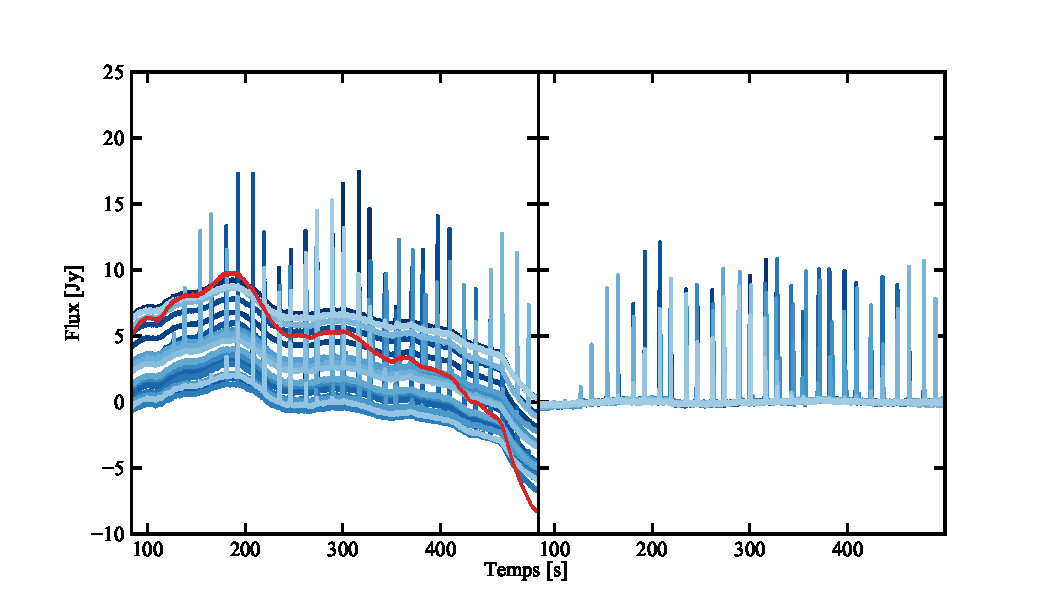
\includegraphics[width=.95\linewidth]{Figures/Chap_decor/toi.pdf}
    \caption{
        \textbf{Gauche:} Données en temps pour 20 détecteurs de la matrice à 150 GHz de NIKA2 lors d'une observation d'Uranus (bleu).
        Le passage de chaque KID sur la planète est visible par les pics d'émission décalés en temps.
        Le mode commun estimé sur les TOI de la matrice entière est représenté en rouge.
    }
    \label{fig:toi_decor_1CM}
\end{figure*}

\subsubsection{Mode commun par boîte électronique} % ---------------------------------- %
Pour la décorrélation illustrée en figure \ref{fig:toi_decor_1CM}, nous avons émis l'hypothèse que le bruit corrélé pouvait être assimilé à un mode commun à tous les KID d'une matrice.
Cette hypothèse repose sur le fait que l'atmosphère est le contaminant dominant dans les données en temps des KID, et que celle-ci est la même pour tous les détecteurs.
Cependant, comme le montre l'équation (\ref{eq:toi}), une autre composante de bruit corrélé est présente dans les données: le bruit dû à l'électronique de lecture.
Celui-ci, par construction, ne présente pas de corrélation entre tous les détecteurs de la matrice, mais seulement entre ceux lus par une même boîte électronique (voir section \ref{sec:kids}, page \pageref{sec:kids}).

Ainsi, à l'issue de la soustraction d'un mode commun atmosphérique, il reste dans les données une composante de bruit corrélé électronique.
Les corrélations entre les KID lors de l'observation d'Uranus présentée en figure \ref{fig:toi_decor_1CM} sont illustrées en figure \ref{fig:toi_corr}.
Sur la gauche sont représentées les corrélations avant soustraction d'un mode commun: tous les détecteurs sont très corrélés entre eux, avec des coefficients de corrélation supérieurs à 99\%.
Sur la droite, on voit les corrélations résiduelles entre les KID après soustraction d'un mode commun calculé sur les TOI de toute la matrice à 150 GHz de NIKA2.
On voit que, si les corrélations sont fortement diminuées -- atteignant des valeurs absolues inférieures à 20\% --, des structures persistent.
En particulier, on remarque deux types de corrélations résiduelles.
Les carrés qui apparaissent corrélés, délimités par des lignes pointillées noires, correspondent aux KID lus par une même boîte électronique.
Les structures carrées plus petites correspondent quant à elles aux détecteurs couplés à la même ligne de lecture.
Ces corrélations montrent l'imperfection de la décorrélation par soustraction d'un seul mode commun pour tous les KID d'une matrice.

\begin{figure*}[t]
    \centering
    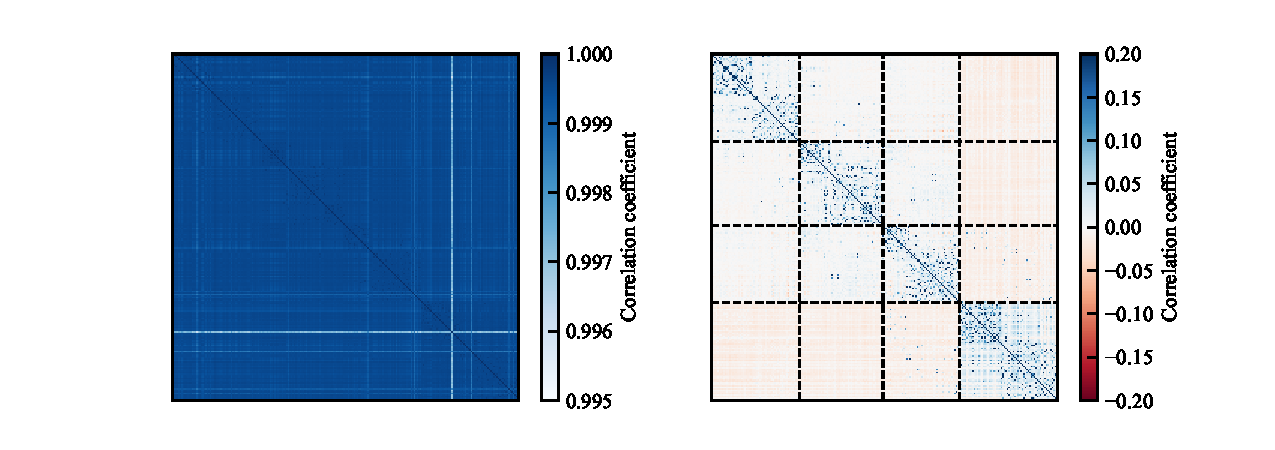
\includegraphics[width=\linewidth, trim={2.3cm .5cm 1.5cm .5cm}, clip]{Figures/Chap_decor/toi_correlation.pdf}
    \caption{
        Matrice de corrélation entre les TOI des détecteurs de la matrice NIKA2 à 150 GHz lors d'une observation d'Uranus.
        \textbf{Gauche:} Corrélations des données brutes, avant soustraction d'un mode commun.
        \textbf{Droite:} Corrélations après soustraction d'un mode commun calculé à partir de tous les détecteurs de la matrice.
        Les lignes noires pointillées délimitent les détecteurs appartenant à chacune des quatre boîtes de l'électronique de lecture de NIKA2.
    }
    \label{fig:toi_corr}
\end{figure*}

Le bruit électronique est en général plus faible que le bruit atmosphérique, bien que les deux composantes puissent avoir une contribution comparable dans le cas d'observations avec d'excellentes conditions météorologiques.
Dans le cas des observations d'Uranus utilisées à titre illustratif en figures \ref{fig:toi_decor_1CM} et \ref{fig:toi_corr}, le bruit électronique est plusieurs ordres de grandeur plus faible que le signal de la planète, d'une dizaine de Jy.
Cependant, pour les observations de l'effet SZ, donc la brillance de surface est au maximum de l'ordre du mJy, le bruit électronique n'est plus négligeable.
Il est donc important, au même titre que pour l'atmosphère, de le retirer des TOI.

Pour ce faire, la procédure d'estimation d'un mode commun détaillée précédemment peut être utilisée, avec une modification notable.
Plutôt que de calculer un mode commun pour tous les détecteurs d'une matrice, la même opération peut être réalisée par groupe de KID, en particulier en les regroupant selon la boîte électronique par laquelle ils sont lus.
Les modes communs résultants contiennent donc à la fois le bruit atmosphérique et le bruit électronique.
D'après l'équation (\ref{eq:toi}), les composantes des TOI restant après soustraction de ce mode commun ne contiennent donc \prior\ plus que le signal d'intérêt et le bruit intrinsèque aux détecteurs.

\subsubsection{Mode commun par groupe de détecteurs corrélés} % ----------------------- %
La décorrélation par ligne de lecture permet donc de tenir compte de deux corrélations différentes entre les KID: celle entre tous les détecteurs d'une matrice, engendrée par le bruit atmosphérique, et celle entre les détecteurs lus par une même électronique de lecture.
D'autres corrélations peuvent être présentes dans les données, mais celles-ci sont difficiles à quantifier: on parle alors de corrélations résiduelles.
On voit notamment dans le panneau droit de la figure \ref{fig:toi_corr} des corrélations entre KID couplés à une même ligne de lecture.
Celles-ci se manifestent par des blocs carrés dans la matrice de corrélation des détecteurs, environ deux fois plus petits que les blocs de KID associés à la même boîte électronique.

Afin d'éliminer au mieux ces corrections résiduelles, on peut procéder à un calcul de mode commun entre détecteurs corrélés.
Pour cela, la matrice de corrélation entre les TOI de tous les détecteurs est calculée.
Les détecteurs sont ensuite groupés par bloc de détecteurs les plus corrélés, indépendamment de toute autre considération (par exemple, de la ligne de lecture à laquelle ils sont couplés).
Un mode commun est calculé pour chacun de ces groupes de KID corrélés, et soustrait de la même façon que pour les méthodes à mode commun par matrice ou par boîte électronique.

Cette méthode est à l'heure actuelle la méthode privilégiée au sein de la collaboration NIKA2, et en particulier pour les observations du grand programme SZ, pour deux raisons principales.
Tout d'abord, comme l'a montré la progression au cours de cette section, elle représente l'aboutissement de la réflexion sur l'exploitation des corrélations entre détecteurs pour retirer le bruit corrélé des données en temps.
De plus, au cours de nombreux tests de différentes méthodes sur des simulations comme sur des données réelles, c'est celle qui a livré les meilleures performances, à la fois en termes de bruit résiduel et de filtrage du signal.
Le filtrage et le bruit résiduel, utilisés à la fois comme métriques pour juger de la qualité du processus de décorrélation et comme outils pour tenir compte des caractéristiques de ce processus lors de l'analyse des cartes, seront discutés en section \mypageref{sec:perf_decor}.
Cette méthode de décorrélation est nommée \textit{common mode one block} dans le pipeline d'analyse des données de la collaboration NIKA2, et décrite dans \cite{perotto_calibration_2020} sous le nom de \textit{most correlated pixels}.

% ------------------------------------------------------------------------------------- %
\subsection{Masquage de source et analyse itérative}\label{sec:mask_decor}

L'estimation du bruit par calcul d'un mode commun permet donc d'obtenir des données en temps dominées par le signal pour chaque détecteur.
Cependant, il faut noter que cette opération est imparfaite: le mode commun des TOI est affecté par la présence de signal dans ces dernières.
Si cet effet est atténué par l'utilisation de la médiane des TOI dans l'estimation des modes communs, il n'est pas complètement annulé.
En particulier, si une proportion significative des détecteurs utilisés dans l'estimation du mode commun passe sur la source au même instant, le mode commun à cet instant contiendra une partie du signal d'intérêt, qui sera soustraite au données et donc perdue dans les cartes.
Le mode commun est donc biaisé par la présence de signal.
Ce biais est d'autant plus important que la source est étendue, puisque la probabilité que deux détecteurs la voient en même temps s'en retrouve augmentée; il est donc particulièrement important dans le cas de l'effet SZ, et \prior\ peu présent pour les sources ponctuelles.
De plus, la méthode d'estimation du mode commun par bloc de détecteurs corrélés augmente par construction l'ampleur de ce biais.
En effet, si la corrélation des TOI pour construire les blocs de données en temps est calculée sans faire la différence entre signal et bruit, des détecteurs voyant simultanément un signal similaire seront corrélés non seulement à cause du bruit, mais également à cause du signal.
Ils auront donc une plus grande corrélation que deux détecteurs voyant la source à des instants différents, et seront groupés pour l'estimation du mode commun.

C'est pourquoi il est important de traiter différemment le signal du bruit au cours de l'estimation du mode commun.
La méthode employée est l'utilisation d'un masque, permettant de ne pas tenir compte des régions contenant du signal dans l'estimation du mode commun.
Ce masque est défini comme la région du ciel contenant du signal astrophysique:
\begin{equation}
    M(x, y) =
        \begin{cases}
            \; 0 \;\text{si du signal est attendu aux coordonnées $(x, y)$}, \\
            \; 1 \;\text{sinon.}
        \end{cases}
\end{equation}
En combinant ce masque avec la matrice de pointage de chaque KID, définie par l'équation (\ref{eq:pointing_matrix}), on peut calculer un masque $M_k(t)$ pour les données en temps de chaque KID,
\begin{equation}
    \label{eq:mask_time}
    M_k(t) = P_k(t, x, y) \times M(x, y) =
        \begin{cases}
            \; 0 \;\text{si du signal est attendu pour le KID $k$ au temps $t$}, \\
            \; 1 \;\text{sinon.}
        \end{cases}
\end{equation}
Le calcul de mode commun décrit précédemment peut donc être réalisé en considérant uniquement les régions des TOI dans lesquelles le masque est non-nul.
Cela permet d'éviter au mode commun d'être biaisé par le signal d'intérêt, puisque les régions contenant du signal ne seront pas considérées dans le calcul du mode commun.

Le calcul du masque requiert donc une connaissance préalable de la région contenant du signal d'intérêt.
Cette opération est délicate, puisque la distinction des contributions du signal et du bruit est l'objectif même de la procédure de décorrélation.
On ne connait donc pas la forme du signal au début de la procédure de décorrélation.
Dans le cadre des observations d'amas de galaxies avec NIKA2, le masque est défini de façon itérative.
Une première estimation du masque est réalisée \prior\ en considérant un disque, centré sur les coordonnées de l'amas, et de rayon suffisamment grand pour inclure tout le signal significatif provenant de l'amas.
La décorrélation par calcul d'un mode commun par blocs de détecteurs corrélés est réalisée dans un premier temps en utilisant ce masque, donnant une première estimation de la distribution du signal astrophysique d'intérêt dans les données en temps de chaque détecteur.
Cette procédure est appliquée pour tous les \textit{scans} réalisés pour l'observation d'un amas.
Les données en temps obtenues, dominées par le signal d'intérêt, sont projetées en cartes du ciel correspondant à chaque \textit{scan}, qui sont ensuite coadditionnées pour obtenir une unique carte de la région de l'amas.
Les procédures de projection et de coaddition seront détaillées en section \mypageref{sec:projec_toi}.
La carte obtenue est utilisée pour déterminer une nouvelle réalisation du masque.
Pour cela, une carte de signal-sur-bruit est calculée comme le rapport entre les cartes de signal astrophysique et de bruit obtenues par la procédure de coaddition.
La région du ciel dans laquelle on détecte un signal astrophysique significatif est utilisée pour mettre à jour le masque $M(x, y)$:
\begin{equation}
    M(x, y) =
        \begin{cases}
            \; 0 \;\text{si le signal-sur-bruit est supérieur à $3\sigma$ aux coordonnées $(x, y)$}, \\
            \; 1 \;\text{sinon.}
        \end{cases}
\end{equation}
La décorrélation est alors répétée avec ce nouveau masque, qui représente une estimation plus fiable de la distribution de signal astrophysique dans la région cartographiée que le masque initial.
La procédure est alors répétée plusieurs fois, en affinant à chaque itération la connaissance du masque grâce à l'itération précédente.
La décorrélation converge alors vers une carte finale, et après quelques ($\sim 5$) itérations, le masque n'évolue plus significativement.

\begin{figure*}[t]
    \centering
    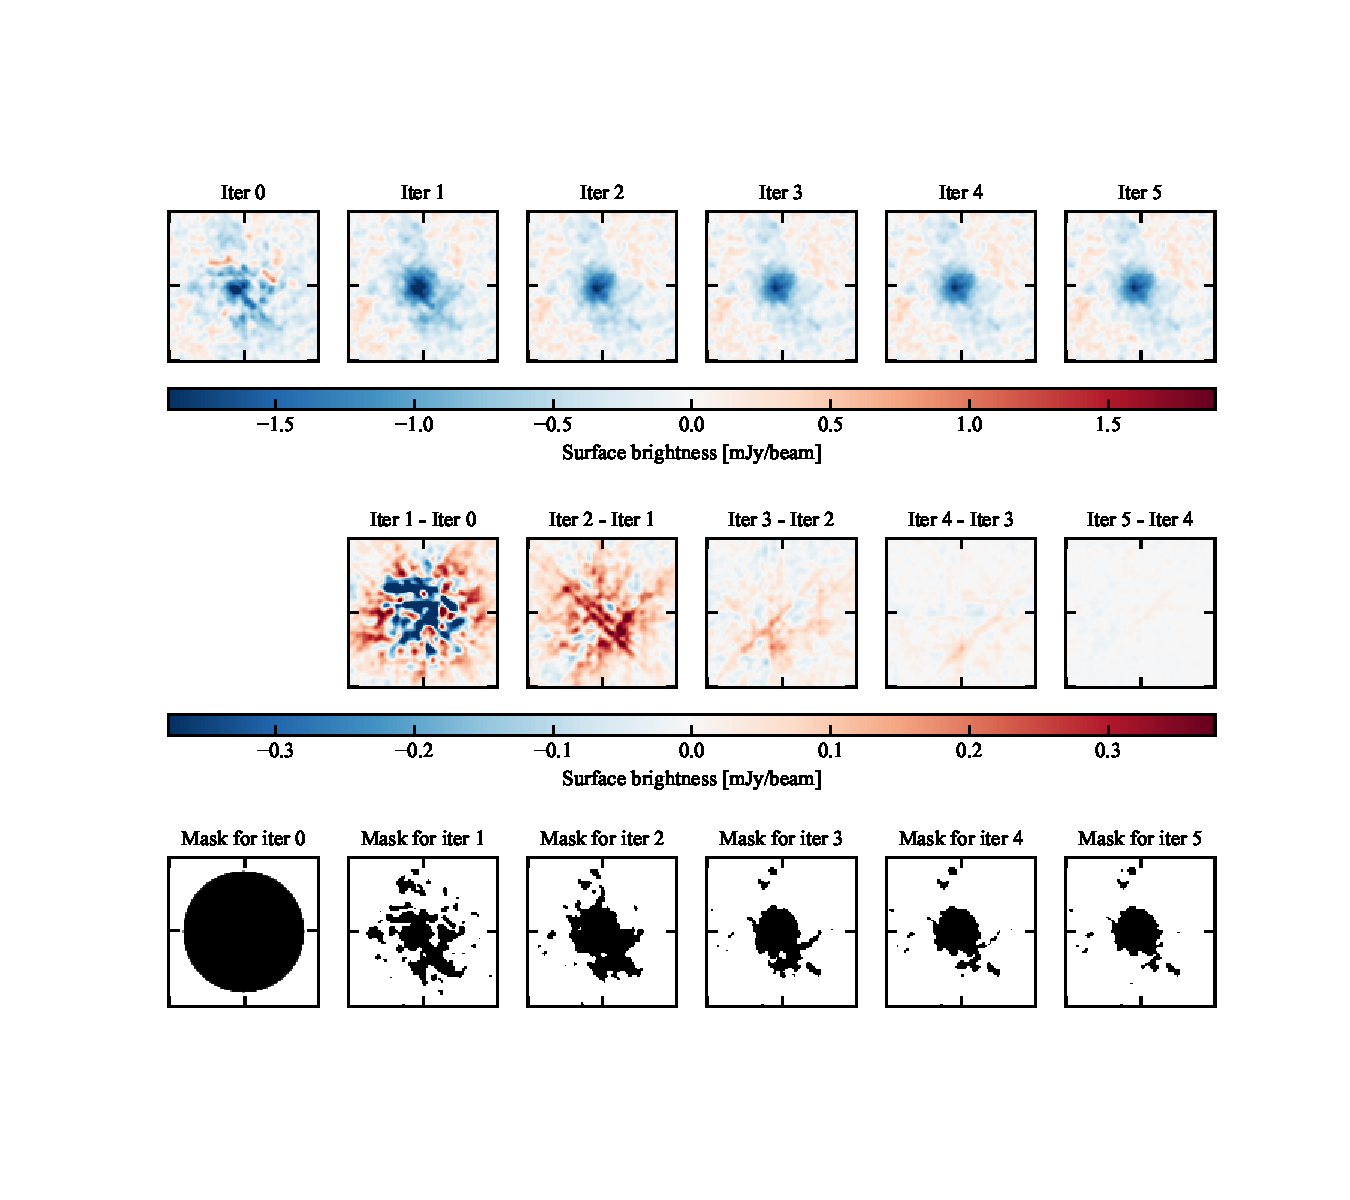
\includegraphics[width=.99\linewidth, trim={2cm 3cm 2cm 3cm}, clip]{Figures/Chap_decor/PSZ2G183_evol_iters.pdf}
    \caption{
        Évolution (de gauche à droite) des résultats avec les itérations de la décorrélation pour les observations NIKA2 de l'amas PSZ2-G183.90+42.99.
        \textbf{Haut:} Carte de brillance de surface obtenue pour chaque itération.
        \textbf{Centre} Différence entre la carte de brillance de surface obtenue pour une itération et pour l'itération précédente.
        \textbf{Bas:} Masque utilisé pour l'évaluation du mode commun pour chaque itération.
    }
    \label{fig:iter_decor}
\end{figure*}

Une décorrélation itérative est illustrée en figure \ref{fig:iter_decor} pour l'amas de galaxies PSZ2-G183.90+42.99.
On voit en haut de la figure, de gauche à droite, l'évolution de la carte de l'amas au fil des itérations.
À partir de la troisième (\guillemotleft Iter 2 \guillemotright), la carte est stable, et n'évolue plus significativement.
Le panneau central montre la différence entre les cartes de deux itérations successives.
On remarque en effet que cette différence converge vers zéro , avec des différences inférieures à $0.1 \;\unit{mJy/beam}$ entre la dernière itération et l'avant-dernière.
Enfin, le panneau bas montre l'évolution du masque utilisé.
On voit que celui-ci mime la morphologie circulaire de l'amas, et que sa forme converge, avec des différences de moins en moins importantes avec les itérations.

% ===================================================================================== %
\section{Des données en temps aux cartes du ciel}\label{sec:projec_toi}

Nous avons vu au cours des sections précédentes comment la procédure de décorrélation permettait d'obtenir des données en temps nettoyées du bruit corrélé, et dominées par le signal d'intérêt.
Il reste donc à projeter ces données pour constituer des cartes du ciel tel qu'observé avec NIKA2.

% ------------------------------------------------------------------------------------- %
\subsection{Projection et cartographie du signal d'intérêt}

La projection utilisée par le \textit{pipeline} de la collaboration NIKA2 est une projection en \textit{nearest grid point}.
Pour cela, une carte de pixels carrés en coordonnées équatoriales et tout d'abord définie.
La taille des pixels est un paramètre de l'analyse, qui peut être choisi.
La taille optimale dépend à la fois de la vitesse de balayage du ciel au cours des observations et de la fréquence d'échantillonnage à laquelle les fréquence des KID sont lues.
En effet, la combinaison de ces deux grandeurs fixe la distance sur le ciel séparant deux échantillons, c'est-à-dire la distance parcourue par le télescope entre deux mesures de fréquence de résonance.
Pour les observations du grand programme SZ de NIKA2, la fréquence d'échantillonnage est $f = 24 \;\unit{Hz}$, et la vitesse de déplacement du télescope de $v = 40 \;\unit{arcsec/s}$.
Le rapport $v/f$ donne donc la distance angulaire séparant deux échantillons consécutifs, qui est de $1.67 \;\unit{arcsec}$.
La taille de pixels est donc choisie comme $3 \;\unit{arcsec}$, permettant à deux échantillons consécutifs de ne jamais être séparés de plus d'un pixel.
Ce critère assure que chaque pixel de la carte soit utilisé pour la projection d'au moins un échantillon.

Une fois la grille de pixels définie, la matrice de pointage $P_k(t, x, y)$ associée à chaque KID est calculée.
La position de chaque détecteur par rapport à un détecteur de référence est connue à chaque instant, comme nous l'avons vu en \mypageref{sec:focal_plane_reconstruction}.
De plus, la position du détecteur de référence dans le ciel étant également connue grâce au pointage du télescope, comme nous l'avons vu en \mypageref{sec:pointing_focus}.
On connait donc, pour chaque mesure de flux réalisée par un KID, la position dans le ciel à laquelle elle a eu lieu.
On peut alors associer chaque mesure de flux au pixel de la carte le plus proche de la position à laquelle elle a été effectuée.

La carte de brillance de surface résultante $I(x, y)$ est obtenue en calculant la moyenne pondérée des mesures associées à chaque pixel:
\begin{equation}
    \label{eq:map_projection}
    I(x, y) = \frac{\sum_{k, t} P_k(t, x, y) \, w_k \; {\rm TOI'}_k(t)}{\sum_{k, t} P_k(t, x, y) \, w_k},
\end{equation}
où ${\rm TOI}'_k(t) = {\rm TOI}_k(t) - B_k(t)$ représente les TOI des détecteurs après soustraction de l'estimation de bruit, c'est-à-dire après la décorrélation. \\
Le poids $w_k$ associé à chaque détecteur $k$ est calculé comme l'inverse de la variance de la TOI du détecteur en dehors du masque $M_k$ (équation \ref{eq:mask_time}).
On a donc:
\begin{equation}
    w_k = \frac{1}{{\rm Var}\,\big[{\rm TOI}_k(t)\big]_{t \,\backslash\, M_k(t) \neq 0}},
\end{equation}
où ${\rm Var}\,[\dots]_{t \,\backslash\, M_k(t) \neq 0}$ représente la variance sur les échantillons $t$ hors du masque, c'est-à-dire la variance hors-source des TOI. \\
Cette pondération permet de donner moins d'importance aux détecteurs dont les données sont toujours fortement bruitées à l'issue de la décorrélation.

% ------------------------------------------------------------------------------------- %
\subsection{Cartes de couverture et de bruit}

Afin de quantifier la couverture des différentes parties du ciel pendant un \textit{scan}, ainsi que le bruit attendu dans les cartes projetées pour ce \textit{scan}, on peut également estimer une carte de couverture et de variance du bruit.
Ces deux cartes sont des sorties naturelles de la procédure de projection.
La carte de couverture, aussi appelée carte de nombre de coups ou de \textit{hits}, représente une cartographie du nombre d'échantillons utilisés pour la projection.
En d'autre termes, il s'agit, pour chaque pixel de la carte, du nombre d'échantillons y ayant été associés par la projection en \textit{nearest grid point}.
Cette carte est obtenue en sommant les matrices de pointages de tous les KID pour tous les échantillons:
\begin{equation}
    \label{}
    N_{\rm hits}(x, y) = \sum_{k, t} P_k(t, x, y).
\end{equation}
Pour un pixel donné, plus ce nombre est élevé, plus le nombre d'échantillons utilisés pour la projection est grand, diminuant ainsi l'incertitude statistique associée au signal en ce point de la carte.

La carte de variance est également un produit de la projection.
En effet, nous avons vu que les échantillons de chaque détecteur étaient pondérés par l'inverse de la variance de sa TOI en dehors de la source.
On peut alors définir une carte de poids, en projetant les poids de chaque détecteur de la même façon que les TOI elles-mêmes sont projetées; ou bien, de façon équivalente, projeter la variance associée à chaque détecteur.
On obtient alors une carte, de pixelisation identique à la carte du signal, représentant la variance des détecteurs utilisés pour la projection du signal dans chaque pixel.
La racine carrée de cette carte donne alors une carte d'écarts-type ou de déviation standard, fournissant une estimation de l'amplitude des fluctuations de bruit, et donc de l'incertitude sur le signal astrophysique en tout point de la carte.

Des exemples de cartes de couverture et de déviation standard de bruit pour un \textit{scan} réalisé au cours des observations de l'amas \act\ dans le grand programme SZ sont présentées dans le panneau haut de la figure \ref{fig:nhits_std_maps}.
On observe la forme rectangulaire des \textit{scans}, caractéristique des observations du grand programme SZ (discutées au paragraphe suivant).
On note également que la carte de couverture montre un nombre plus important de coups dans le centre de la carte qu'en périphérie.
Cette inhomogénéité de couverture s'explique par le fait que plus de détecteurs passent dans les régions du centre de la carte, pour des raisons géométriques, alors que sa périphérie n'est visitée que par un plus faible nombre de KID.
Pour les mêmes raisons, la déviation standard du bruit est plus élevée dans les régions externes de la carte, entraînant des observations de meilleure qualité au centre.
Une analyse détaillée des propriétés de cet amas sera présentée au chapitre \ref{chap:actj0215}.

% ------------------------------------------------------------------------------------- %
\subsection{Coaddition de cartes} \label{sec:map_coadd}

Tout comme la carte de brillance de surface associée à un \textit{scan} est calculée par une moyenne pondérée des signaux reçus par les KID, la combinaison de plusieurs \textit{scans} permet de construire une carte de brillance de surface en calculant la moyenne pondérée des cartes de ces derniers.
La carte de brillance résultant de la combinaison de $n$ \textit{scans}, donc les cartes de brillance de surface individuelles $I_s(x,y)$ sont calculées par l'équation (\ref{eq:map_projection}), est donnée par:
\begin{equation}
    \label{eq:map_coadd}
    I_{\rm tot}(x, y) = \frac{\sum_{s=1}^{n} w_s(x, y) \, I_s(x, y)}{\sum_{s=1}^{n} w_s(x, y)},
\end{equation}
où les poids $w_s(x, y)$ sont définis pour chaque carte à partir de la carte de couverture $N_{\rm hits}(x, y)$ et de la variance de la carte de brillance de surface en dehors du masque de la source:
\begin{equation}
    \label{eq:coadd_weights}
    w_s(x, y) = \frac{N_{{\rm hits}, s}(x, y)}{V \, \big[ I_s(x, y) \times \sqrt{N_{{\rm hits}, s}(x, y)} \big]_{(x, y) \,\backslash\, M(x, y) \neq 0}}.
\end{equation}
Tout comme la pondération par la variance des TOI nous a permis de donner moins d'importance aux détecteurs bruités, cette pondération permet de donner moins d'importance dans la carte finale aux \textit{scans} dans lesquels le bruit est toujours important après la décorrélation.
Le terme $\sqrt{N_{{\rm hits}, s}(x, y)}$ au dénominateur permet de normaliser la carte au temps passé par pixel.

Nous avons vu au chapitre précédent que la stratégie de \textit{scan} utilisée pour les observations du grand programme SZ de NIKA2 était basée sur une succession de groupes de quatre \textit{scans}, réalisés à des angles de $0$\textdegree, $45$\textdegree, $90$\textdegree, et $135$\textdegree par rapport à l'axe des ascensions droites.
La procédure de coaddition est donc particulièrement importante dans ce contexte.
Le panneau bas de la figure \ref{fig:nhits_std_maps} montre les cartes de couverture et de déviation standard du bruit obtenues par coaddition de quatre \textit{scans} de l'amas \act, dont celui présenté dans le panneau haut de la figure.
Les observations faites sur le panneau haut (voir section précédente) restent valides: le centre de la carte bénéficie d'une meilleure couverture, et donc d'une déviation standard de bruit plus faible.
On voit également que la combinaison de \textit{scans} dans quatre angles différents a eu pour effet d'augmenter la couverture dans la carte (puisqu'on considère quatre \textit{scans} au lieu d'un seul), mais également de la rentre plus isotrope.
De même, le bruit dans la carte coadditionnée est plus bas, et reste bas dans une grande région à symétrie circulaire.
C'est là l'objectif de l'utilisation de \textit{scans} dans plusieurs directions mise en place pour les observations du grand programme SZ de NIKA2, en plus de l'optimisation du filtrage, que nous discuterons en section \mypageref{sec:transfer_function}.

\begin{figure*}[t]
    \centering
    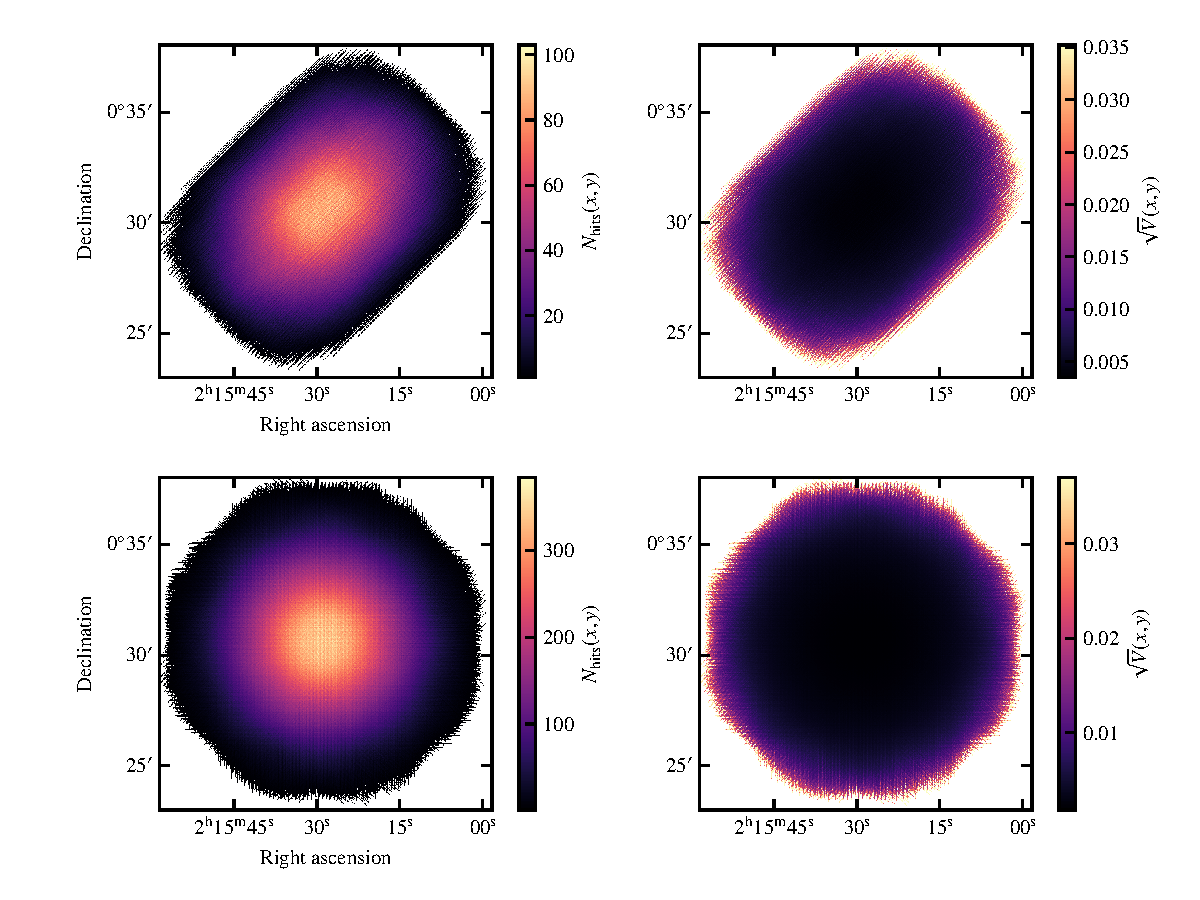
\includegraphics[width=\linewidth]{Figures/Chap_decor/scans.pdf}
    \caption{
        \textbf{Haut:} carte de couverture (\textit{gauche}) et de déviation standard du bruit (\textit{droite}) à 150 GHz pour un \textit{scan} du grand programme SZ de NIKA2.
        \textbf{Bas:} Mêmes cartes pour la combinaison de quatre \textit{scans} dans quatre orientations différentes, incluant le \textit{scan} du panneau haut.
    }
    \label{fig:nhits_std_maps}
\end{figure*}

% ===================================================================================== %
\section{Performance de la décorrélation}\label{sec:perf_decor}

Quelle que soit la méthode choisie pour la procédure de décorrélation, celle-ci est toujours imparfaite.
Nous avons vu que la décorrélation avait deux objectifs, qui sont de retirer un maximum de bruit corrélé des données en temps sans porter atteinte au signal astrophysique d'intérêt.
Par conséquent, on quantifie la performance de la procédure au travers de critères évaluant l'atteinte de ces deux objectifs: le bruit corrélé résiduel, et le filtrage du signal.
Ces deux quantités seront ensuite utilisées au cours de l'analyse des données de NIKA2 afin de tenir compte des caractéristiques de la décorrélation.

% ------------------------------------------------------------------------------------- %
\subsection{Bruit corrélé résiduel}\label{sec:noise_pk}

À l'issue de la procédure de décorrélation, une partie du bruit reste inévitablement présente dans les données en temps.
Nous avons vu précédemment qu'une partie de ce bruit était le bruit blanc intrinsèque à chaque détecteur, ne pouvant par nature pas être soustrait des données en temps.
En réalité, une partie du bruit corrélé dû à l'atmosphère et à l'électronique reste également présent.
La présence de ce bruit corrélé résiduel est donc une indication de l'imperfection de la méthode de décorrélation.
Puisque ce bruit reste dans les données en temps après la décorrélation, il est projeté dans les cartes de brillance de surface au même titre que le signal astrophysique.
De plus, puisqu'il est corrélé, il peut faire apparaître des structures de bruit dans les cartes, pouvant être faussement interprétées comme du signal d'intérêt.
Il est donc important de connaitre le comportement de ce bruit en vue de la mesure des propriétés des amas de galaxies à partir des observations avec NIKA2.

L'information pertinente sur le bruit corrélé résiduel est présente dans son spectre de puissance.
L'évaluation de celui-ci ne peut pas avoir lieu directement dans les données NNIKA2, puisque celles-ci contiennent également du signal d'intérêt.
Cependant, il est possible d'utiliser les cartes de demi-différences entre les \textit{scans}.
Pour cela, on réalise la coaddition des $n$ cartes des différents \textit{scans} d'après:
\begin{equation}
    I'(x, y) = \frac{\sum_{s=1}^{n} w_s(x, y) \, I_s(x, y) \times (-1)^s}{\sum_{s=1}^{n} w_s(x, y)},
\end{equation}
où les poids $w_s$ sont les mêmes que pour la coaddition des \textit{scans}, calculés par l'équation (\ref{eq:coadd_weights}). \\
Ainsi, la carte d'un \textit{scan} sur deux se voit multipliée par $(-1)$ dans la coaddition.
Puisque le signal astrophysique est \prior\ la seule composante des cartes constante d'un \textit{scan} à l'autre, il est complètement annulé\footnotemark\ dans la carte $I'(x, y)$.
En revanche, le bruit corrélé pouvant indifféremment être positif ou négatif, sa structure n'est pas modifiée au cours de l'opération.
\footnotetext{On note la nécessité d'un nombre pair de \textit{scans} dans cette procédure, sans quoi le signal ne peut complètement s'annuler.
De même, il est nécessaire d'ordonner les \textit{scans} par angle lors de la coaddition, afin de ne pas systématiquement ajouter ou soustraire les cartes obtenues à un angle donné, ce qui crée des structures de bruit différentes.}
On obtient ainsi une carte, vide de tout signal d'intérêt, contenant seulement du bruit dont les propriétés sont les mêmes que celles du bruit présent dans la carte de signal obtenue par coaddition.

Le spectre de puissance du bruit résiduel est calculé sur la carte de demi-différences, normalisée par la carte de déviation standard du bruit:
\begin{equation}
    \label{eq:noise_power_spectrum}
    P_{\rm bruit}(k) = \left| \, F \left( \frac{I'(x, y)}{\sqrt{V}(x, y)} \right) \, \right|^2,
\end{equation}
où $F$ représente l'opération de transformée de Fourier. \\
Cette normalisation permet de tenir compte de la plus grande amplitude de bruit attendue dans les bords des cartes, du fait de la couverture plus faible dans ces régions.
La forme du spectre de puissance nous renseigne sur la corrélation du bruit résiduel.
Si ce dernier est blanc, c'est-à-dire ne présente pas de corrélations résiduelles, son spectre de puissance doit être plat.
À l'inverse, le spectre de puissance d'un bruit fortement corrélé à grande échelle se manifeste comme une fonction en loi de puissance, $P(k) \propto k^{-\alpha}$.
Pour la décorrélation \textit{common mode one block} réalisée sur les amas du grand programme SZ, c'est ce dernier comportement qui est observé.
Nous verrons par exemple au chapitre \ref{chap:actj0215} que le bruit résiduel dans les observations de l'amas \act\ est très corrélé, comme en atteste le spectre de puissance présenté en figure \ref{fig:act:tf_noise}.

C'est pourquoi la présence de bruit corrélé doit être prise en compte au cours des exploitations des observations d'amas de galaxies par NIKA2.
Nous verrons au chapitre suivant que cette prise en compte est possible au travers de la matrice de covariance du bruit résiduel.
Celle-ci peut être calculée à partir du spectre de puissance comme suit:
\begin{enumerate}[leftmargin=*]
    \item Un grand nombre ($N \sim 10^5$) de cartes de bruit blanc est généré.
        Dans chacune des cartes, chaque pixel est tiré aléatoirement dans une distribution gaussienne de moyenne $0$ et de variance $1$.
    \item Chacune de ces cartes est convoluée par le spectre de puissance du bruit calculé par l'équation (\ref{eq:noise_power_spectrum}).
        Les cartes résultantes sont des réalisations de bruit normalisées suivant le spectre de puissance d'entrée.
    \item Chacune des cartes est ensuite multipliée par la carte de déviation standard du bruit $\sqrt{V}(x, y)$.
        Les cartes résultantes sont des réalisations de bruit résiduel dont l'amplitude et les corrélations sont les mêmes que dans la carte de demi-différences.
        Chaque carte, de dimension $(n \times n)$, est déroulée en un vecteur de dimension $(n^2 \times 1)$.
    \item La matrice de covariance des $N$ vecteurs est calculée.
\end{enumerate}
Pour une carte d'entrée de dimensions $(n \times n)$ pixels, le résultat est une matrice de taille $(n^2 \times n^2)$, dans laquelle chaque élément $(i, j)$ représente la covariance du bruit dans les pixels $i$ et $j$ de la carte.
Nous verrons au chapitre suivant que c'est cette matrice qui est utilisée dans la fonction de vraisemblance multivariée de l'ajustement des données NIKA2 par un modèle de propriétés physiques du milieu intra-amas, afin de tenir compte de la corrélation du bruit résiduel.
Elle sera utilisée au travers d'une fonction de vraisemblance gaussienne multivariée, discutée en section \mypageref{sec:panco:likelihood}.

\begin{figure*}[t]
    \centering
    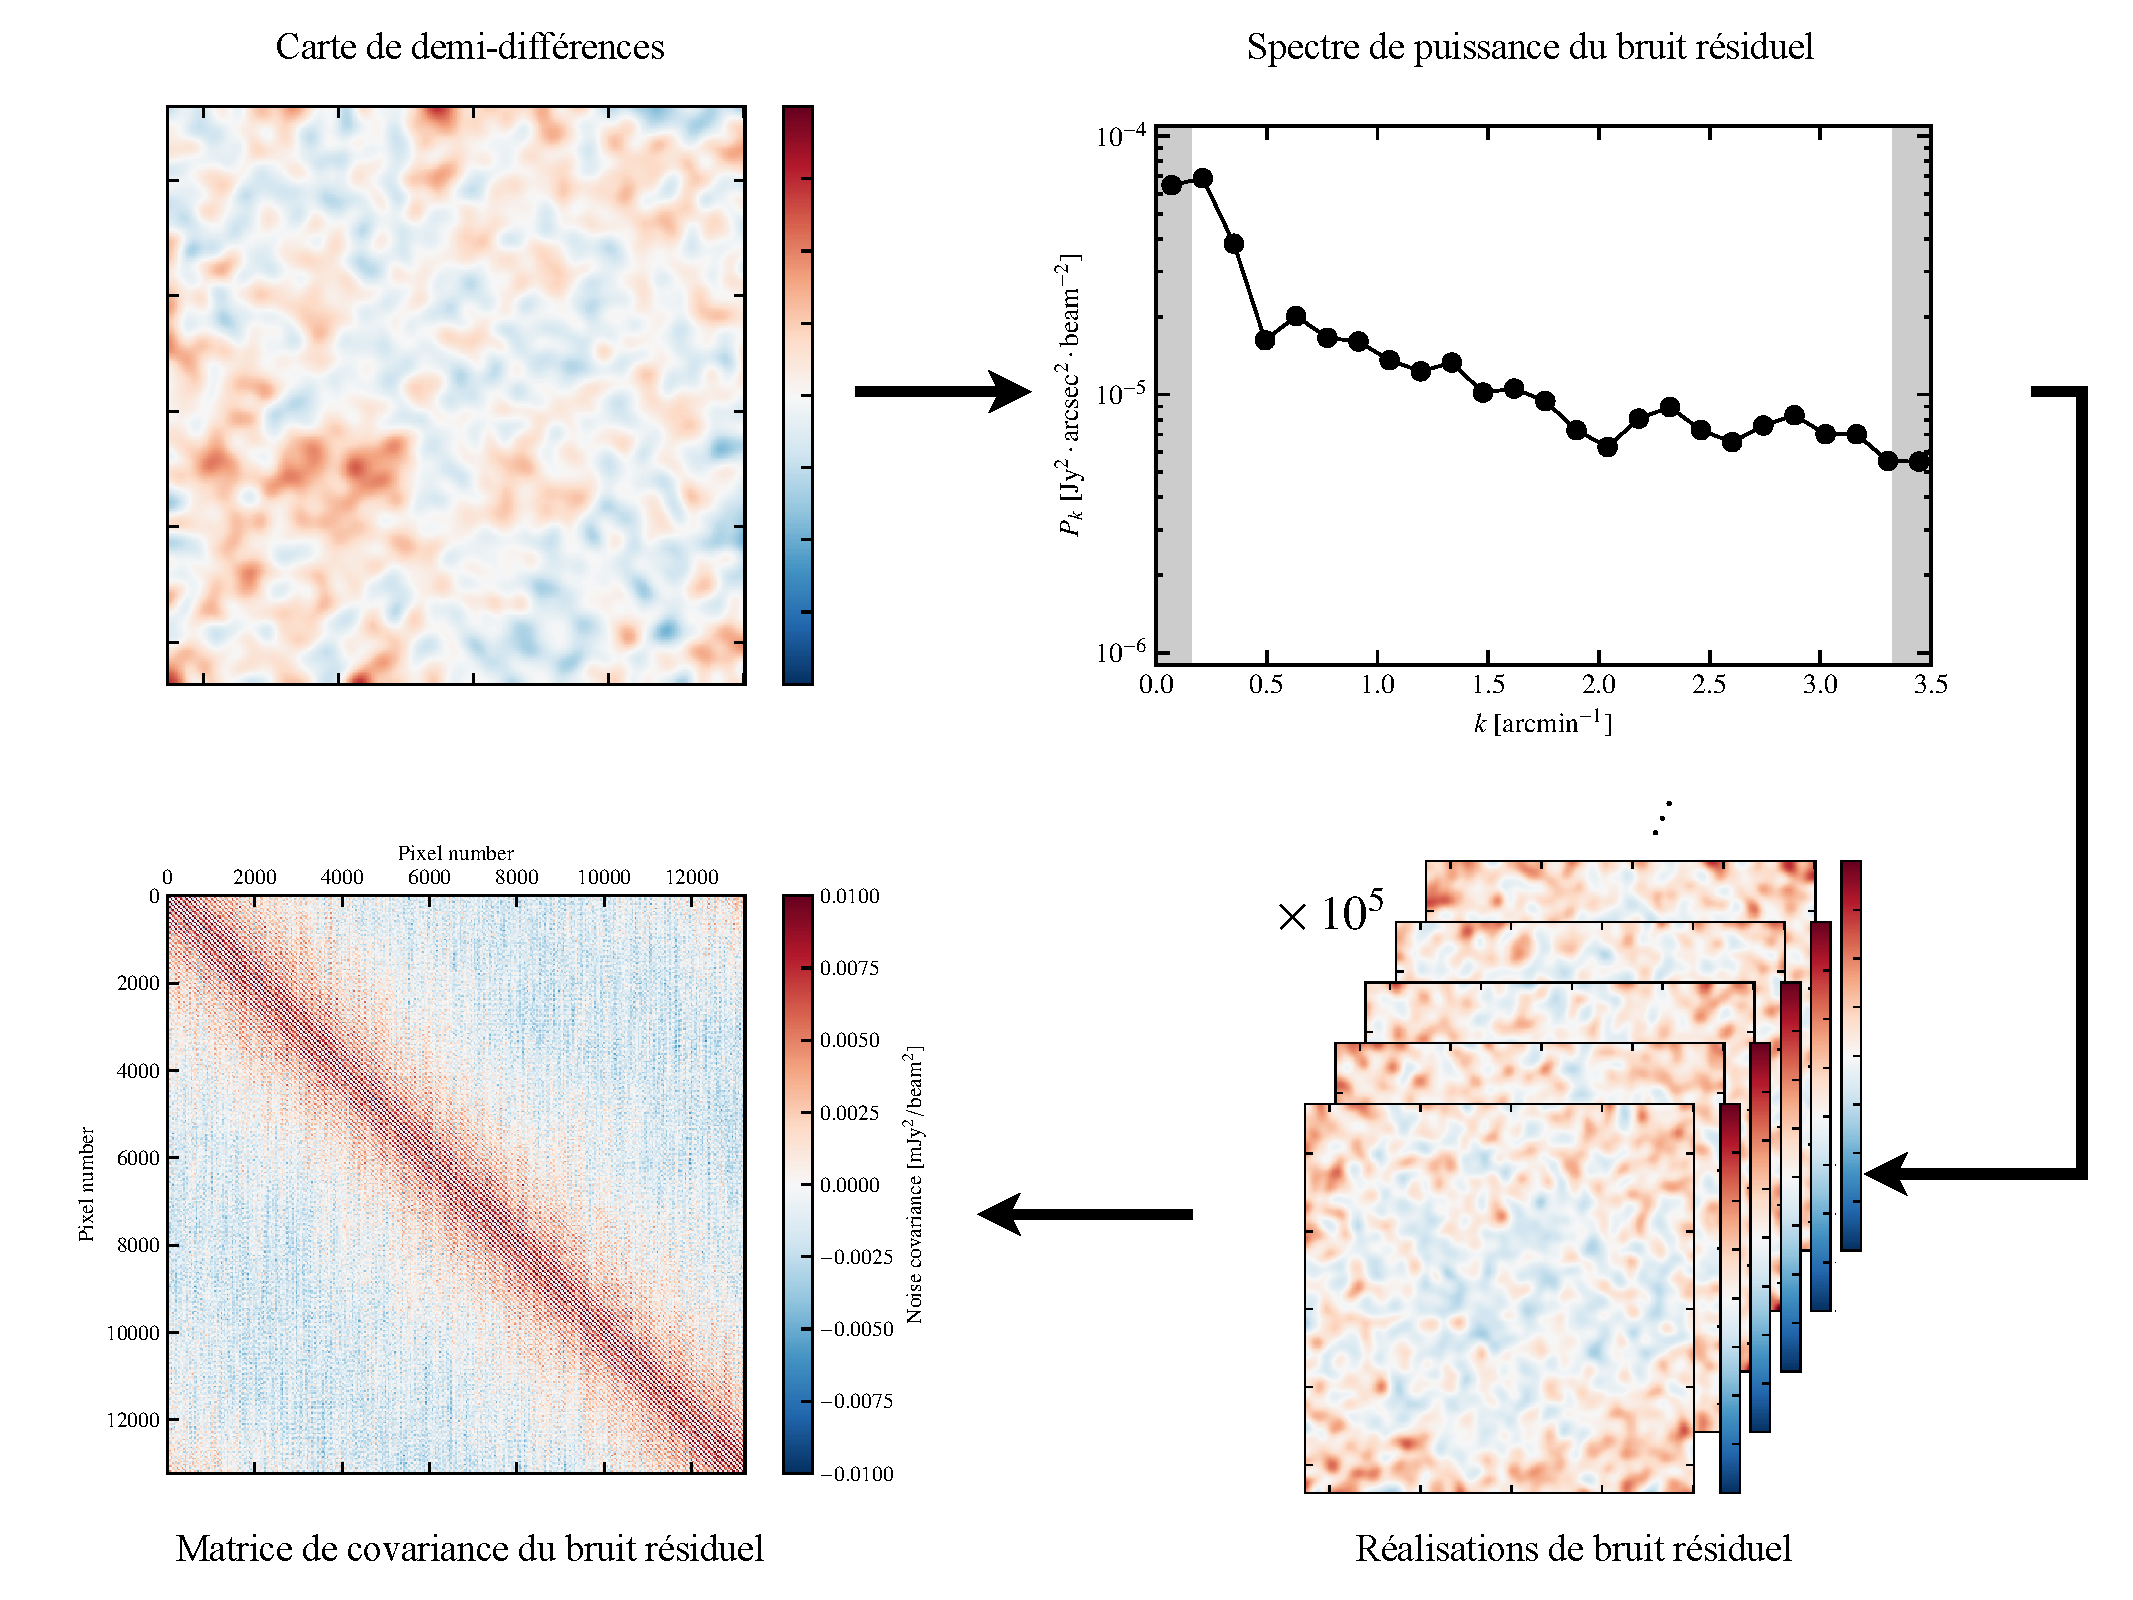
\includegraphics[width=.99\linewidth, page=1]{Figures/Chap_decor/schema_pk_tf.pdf}
    \caption{
        Illustration du calcul de la matrice de covariance du bruit résiduel pour la décorrélation \textit{common mode one block} de l'amas PSZ2-G183.90+42.99 (voir figure \ref{fig:iter_decor}).
        La carte de demi-différences (\textit{haut gauche}) est utilisée pour calculer le spectre de puissance du bruit résiduel (\textit{haut droit}), à son tour utilisé pour générer des réalisations de bruit corrélé de même spectre de puissance (\textit{bas droit}).
        La covariance de ces réalisations donne la matrice de covariance pixel-à-pixel du bruit résiduel (\textit{bas gauche}).
    }
    \label{fig:noise_pk_schema}
\end{figure*}

La procédure d'estimation du bruit résiduel et de sa matrice de covariance est présentée en figure \ref{fig:noise_pk_schema}.
Le cas choisi pour l'illustration est la décorrélation \textit{common mode one block} des observations de l'amas PSZ2-G183.90+42.99, dont le processus itératif est représenté en figure \ref{fig:iter_decor}.
Le spectre de puissance du bruit résiduel (haut droite de la figure) n'est pas plat, indiquant un bruit résiduel corrélé à grande échelle.
Par conséquent, la matrice de covariance du bruit (bas gauche) n'est pas diagonale.
Dans le cas où le bruit résiduel est proche d'un bruit blanc, les corrélations du bruit entre deux pixels différents de la carte sont faibles, et les éléments extra-diagonaux de la matrice de covariance sont négligeables.
Ce comportement traduirait une décorrélation parfaite.
De plus, comme nous le verrons au chapitre suivant, ce comportement est idéal, car il permet de ne pas tenir compte de la matrice de covariance du bruit lors de l'ajustement des propriétés des amas à partir des observations NIKA2, ce qui accélère grandement le processus.

% ------------------------------------------------------------------------------------- %
\subsection{Filtrage du signal}\label{sec:transfer_function}

Si la décorrélation ne permet pas de retirer complètement le bruit corrélé des données en temps, elle est aussi imparfaite du point de vue de la conservation du signal.
En effet, nous avons vu en section \ref{sec:mask_decor} que le masque utilisé pour éviter le biais dû au signal dans l'estimation du mode commun était défini comme la région du ciel dans laquelle le rapport signal sur bruit était supérieur à $3\sigma$.
Par construction, tout signal moins significatif n'est pas protégé par ce masque, et peut être inclus dans le mode commun.
Il est alors soustrait comme du bruit, ce qui induit un filtrage du signal d'intérêt.
Par ailleurs, nous avons vu que le masque était défini de façon itérative, en commençant avec un masque circulaire assez grand pour englober le signal.
Il ne s'agit toutefois pas simplement de définir un masque le plus grand possible pour masquer une grande portion de la carte, puisqu'une couverture du ciel minime entraînera un mode commun estimé sur peu de détecteurs, et donc potentiellement une mauvaise estimation de bruit.
Ces défauts sont donc d'autant plus importants que la source observée est spatialement étendue.
Les amas de galaxies observés dans le cadre du grand programme SZ de NIKA2 étant grands devant le lobe de l'instrument (voir section \ref{sec:lpsz}), ils sont affectés par ce filtrage.
Il est donc nécessaire de connaitre les propriétés de ce filtrage, afin de pouvoir faire le lien entre le signal SZ réel associé à l'amas et le signal détecté, faute de quoi les propriétés physiques mesurées seront biaisées.

Ce filtrage est estimé par la fonction de transfert de l'analyse.
Celle-ci est évaluée par la mesure du filtrage subi par un signal connu lorsque celui-ci est soumis à la procédure de décorrélation.
Pour l'analyse des données associées à un amas, une fois la décorrélation terminée, une carte de l'effet SZ dû à l'amas est simulée par intégration d'un profil de pression universel le long de la ligne de visée.
Cette carte est projetée sur la même grille pixélisée que la carte de brillance de surface NIKA2.
Une réalisation de bruit blanc, d'amplitude largement inférieure au signal SZ simulé, est ajoutée à la carte afin d'éviter la présence de zéros dans la carte et dans son spectre de puissance.
L'importante de ce bruit sera discutée par la suite.
La carte simulée obtenue $S_{\rm in.}$ est ensuite convertie en données en temps pour chaque détecteur grâce à la matrice de pointage de ces derniers.
Les données en temps ainsi obtenues, entièrement dominées par le signal simulé, sont ajoutées aux données réelles.
Cette somme forme donc des TOI pour chaque détecteur contenant les différents contaminants caractéristiques des observations avec NIKA2, le signal astrophysique d'intérêt, et le signal simulé.

Les données en temps ainsi obtenues sont soumises à la même procédure de décorrélation que les données NIKA2 ne contenant pas le signal simulé.
La procédure itérative n'est pas nécessaire, puisqu'elle vise seulement à définir le masque le plus adapté à la protection du signal d'intérêt.
Ainsi, la procédure de décorrélation est réalisée sur les TOI contenant le signal simulé en considérant le masque utilisé pour la dernière itération de la décorrélation des données brutes.
De cette façon, le traitement subi par les données contenant le signal simulé est identique à celui subi par les données brutes.
On peut donc supposer que le filtrage subi par le signal simulé est identique à celui subi par le signal astrophysique d'intérêt.

La carte de signal simulé reconstruit $S_{\rm out.}$ est ensuite calculé comme la différence entre la carte issue de la décorrélation des données en temps contenant le signal simulé et celle issue de la décorrélation des données brutes (ne contenant pas de signal simulé).
La fonction de transfert de l'analyse ${\rm TF}(k)$, quantifiant le filtrage subi par le signal simulé, est calculée comme le rapport entre les spectres de puissance des cartes de signal simulé avant et après la décorrélation:
\begin{equation}
    \label{eq:transfer_function}
    {\rm TF}(k) = \frac{\big| F(S_{\rm out.}) \big|^2}{\big| F(S_{\rm in.}) \big|^2}
\end{equation}
Puisque le processus subi par le signal simulé est identique à celui subi par le signal astrophysique d'intérêt, cette fonction de transfert représente un bon estimateur du filtrage subi par ce dernier au cours de la décorrélation ne contenant pas de signal simulé.
L'intérêt de l'ajout de bruit blanc dans la carte de signal simulé $S_{\rm in.}$ apparaît clairement dans l'équation (\ref{eq:transfer_function}).
Si cette étape n'était pas réalisée, il existe un risque que le spectre de puissance de la carte présente des zéros.
Ce dernier étant au dénominateur de l'équation (\ref{eq:transfer_function}), la fonction de transfert peut diverger.

\begin{figure*}[t]
    \centering
    \includegraphics[width=.99\linewidth, page=2]{Figures/Chap_decor/schema_pk_tf.pdf}
    \caption{
        Illustration du calcul de la fonction de transfert pour la décorrélation \textit{common mode one block} de l'amas PSZ2-G183.90+42.99 (voir figure \ref{fig:iter_decor}).
        Le rapport entre les spectres de puissance d'une carte simulée d'entrée ($S_{\rm in.}$, \textit{haut}) et de la carte après décorrélation ($S_{\rm out.}$, \textit{bas}) donne la fonction de transfert de la décorrélation.
    }
    \label{fig:tf_schema}
\end{figure*}

Le processus d'estimation de la fonction de transfert pour la décorrélation des observations de l'amas PSZ2-G183.90+42.99 est schématisé en figure \ref{fig:tf_schema}.
La fonction de transfert résultante, représentée à droite de la figure, est caractéristique de la décorrélation \textit{common mode one block} des observations NIKA2 d'amas de galaxies.
Elle est caractérisée par un filtrage des grandes échelles angulaires ($k < 0.5 \;\unit{arcmin^{-1}}$), résultant en une suppression quasi-totale du signal aux échelles plus grandes que le champ de vue instantané de NIKA2 ($6.5 \;\unit{arcmin}$), représentées par la région grisée à gauche de la figure.
En revanche, les échelles angulaires plus petites sont bien conservées, avec un filtrage proche de $1$.
Nous verrons dans le chapitre suivant que cette fonction de transfert est utilisée lors de la mesure des propriétés thermodynamiques du milieu intra-amas à partir des observations NIKA2 des amas du grand programme SZ, afin de tenir compte du filtrage induit par la décorrélation.

% ===================================================================================== %
\section{Contamination par des sources ponctuelles}
\label{sec:decor:pstools}

Nous avons vu au chapitre \ref{chap:nika2} que l'effet SZ pouvait être mesuré avec NIKA2 par le décrément en brillance de surface dans la carte à 150 GHz.
Ce signal peut être affecté par des sources ponctuelles, de flux positif qui compense partiellement ou totalement le décrément.
Afin d'obtenir des contraintes non-biaisées sur le signal SZ d'un amas -- et donc sur ses propriétés thermodynamiques -- il est donc nécessaire de traiter cette contamination en estimant le flux des sources.
Celui-ci ne peut par construction pas être mesuré directement dans la carte NIKA2 à 150 GHz, puisqu'il est dégénéré avec le décrément SZ inconnu.
Il est donc nécessaire de s'appuyer sur des données externes.

Un estimateur du flux d'une source est donné par l'évolution de son émission avec la fréquence d'observation, qui est quantifiée par son spectre (SED, pour \textit{Spectral Energy Distribution}).
Le logiciel \texttt{PSTools} a été développé dans le cadre de cette thèse, et permet d'ajuster ce flux pour des sources sub-millimétriques à partir d'un catalogue de sources et des données NIKA2.
Ce logiciel a été documenté et mis à disposition de la collaboration NIKA2, devenant l'outil principal d'estimation de la contamination des cartes SZ obtenues avec NIKA2 par des sources sub-millimétriques.
Cette section décrit la procédure employée et implémentée dans \texttt{PSTools}; son utilisation dans le cadre de l'analyse des propriétés de l'amas \act\ sera présentée au chapitre \ref{chap:actj0215}.

% ------------------------------------------------------------------------------------- %
\subsection{Données d'entrée}

Les sources ponctuelles contaminant le signal SZ peuvent être des sources d'avant-plan, d'arrière-plan, ou même des galaxies membres de l'amas.
Dans tous les cas, ces sources peuvent être classifiées en deux catégories.
D'une part, elle peuvent être des galaxies poussiéreuses émettant dans le domaine sub-millimétrique (SMG pour \textit{submillimeter galaxies}), avec un flux croissant avec la fréquence dans le domaine couvert par les observations NIKA2.
Elles peuvent également être des sources radio, présentant une émission plus forte à basse fréquence\footnotemark.
\footnotetext{Notons que cette distinction entre galaxie poussiéreuse et source radio est une simplification, le spectre d'émission de la poussière présentant une composante d'émission radio.}
Les SMG sont plus simples à identifier avec NIKA2, puisque leur flux est plus élevé dans la bande à 260 GHz, où le signal SZ n'est en général pas détectable.

Afin de mesurer le spectre d'une source, la connaissance de son flux dans une large gamme de fréquences est nécessaire.
\texttt{PSTools} permet de traiter la contamination due à des sources submillimétriques détectées par l'instrument SPIRE à bord du satellite \textit{Herschel} \cite{griffin_herschel-spire_2010}.
Nous utilisons la combinaison des mesures de flux dans chacune des bandes de SPIRE (250, 350, et 500 ${\rm \mu m}$, soit 1200, 860, et 600 GHz, respectivement) et dans la bande à 260 GHz de NIKA2, dans laquelle le signal SZ est négligeable devant le bruit et le flux des sources ponctuelles.
Il est également possible d'utiliser les flux des sources à plus haute fréquence dans les bandes passantes de l'instrument PACS à bord de \textit{Herschel} \cite{poglitsch_photodetector_2010}, lorsque ceux-ci sont publics.
Par la suite, nous considèrerons le cas où seules des données SPIRE sont disponibles, cas bien plus fréquent pour les amas du grand programme SZ.

Un schéma du fonctionnement de \texttt{PSTools} est présenté en figure \ref{fig:pstools_schema}.
Les données d'entrée sont donc un catalogue de sources avec leurs positions et flux dans les trois bandes de SPIRE d'une part, et les données NIKA2 à 260 GHz d'autre part, incluant la carte de signal, de bruit, et la fonction de transfert associée.
Dans la suite, nous présentons les trois grandes étapes de l'analyse, représentées en bleu-vert sur la figure \ref{fig:pstools_schema}, et les illustrons pour des sources considérées dans l'analyse de l'amas \act, présentée au chapitre \ref{chap:actj0215}.

\begin{figure*}[t]
    \centering
    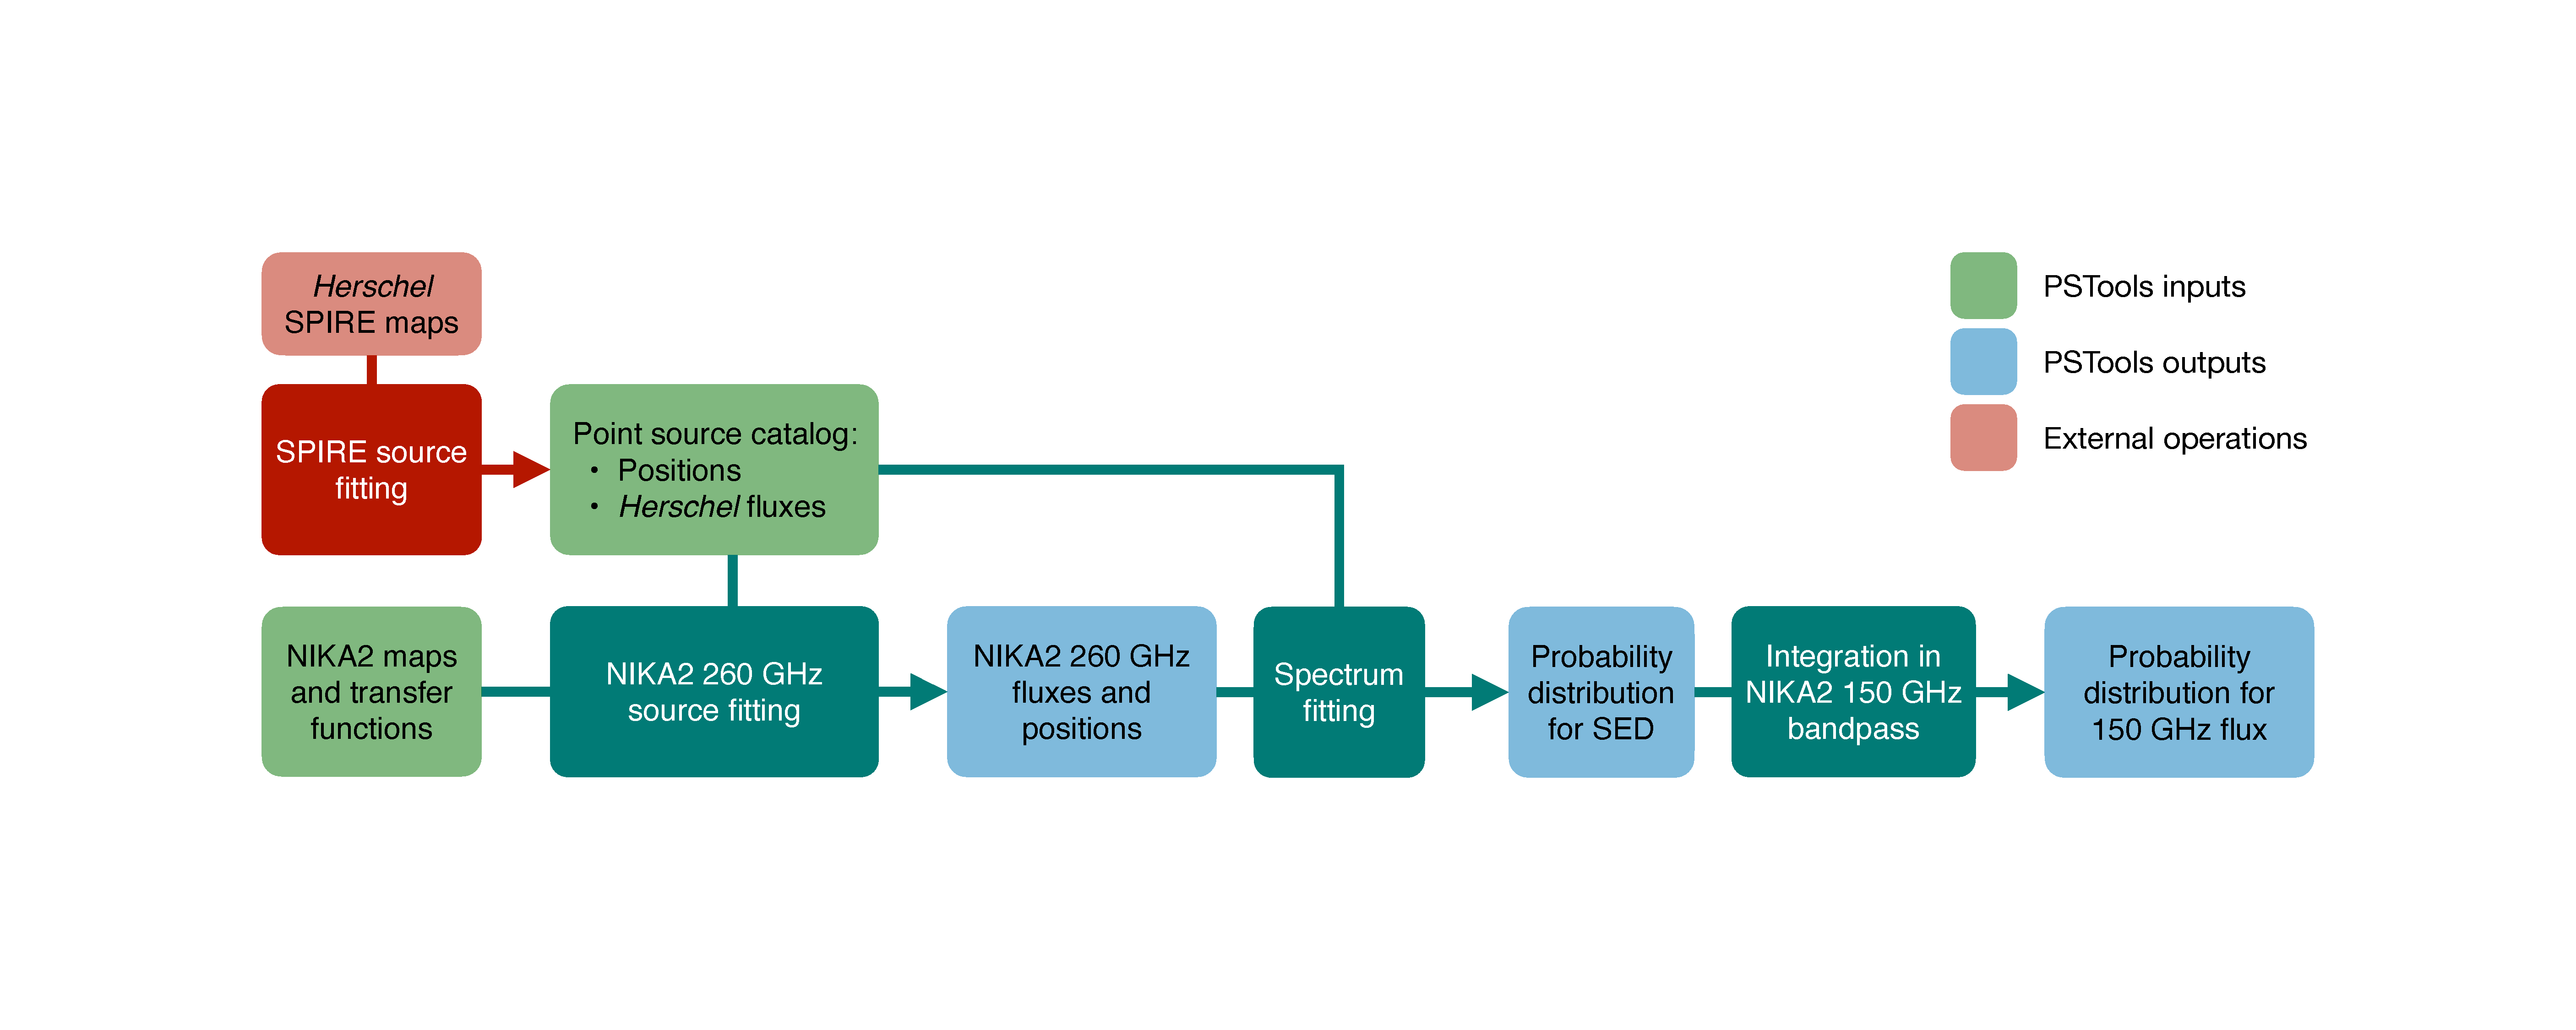
\includegraphics[width=\linewidth, trim={8cm, 7cm, 8cm, 7cm}, clip]{Figures/Chap_decor/PSTools.pdf}
    \caption{
        Schéma illustrant le fonctionnement de \texttt{PSTools}.
        Les données d'entrée sont représentées en vert, et les données de sortie en bleu.
        La partie rouge représente les opérations externes au logiciel, c'est-à-dire la détection des sources dans les cartes SPIRE.
    }
    \label{fig:pstools_schema}
\end{figure*}

% ------------------------------------------------------------------------------------- %
\subsection{Mesures de coordonnées et flux à 260 GHz}

Le flux de chaque source à 260 GHz et sa position sont mesurés dans la carte NIKA2 à cette fréquence.
Pour cela, un modèle de lobe de NIKA2 est ajusté dans une portion carrée de la carte, centrée sur la position de détection de chaque source dans SPIRE.
L'évolution de la mesure du flux des sources avec la taille de cette portion a été étudiée, montrant de meilleurs résultats pour des tailles d'environ une minute d'arc.
Le lobe est modélisé par une Gaussienne de largeur à mi-hauteur fixée à $\mathrm{FWHM} = 12.5$'', en accord avec le modèle utilisé pour l'étalonnage des cartes \cite{perotto_calibration_2020}, avec une amplitude et une position libres, ainsi qu'un éventuel niveau zéro.
L'ajustement est réalisé à l'aide de la librairie Python \texttt{iminuit} \cite{hans_dembinski_scikit-hepiminuit_2020}, et l'amplitude de la Gaussienne ajustée livre une estimation du flux de la source à 260 GHz.
Lorsque deux sources sont proches, elles sont ajustées simultanément dans la même portion de carte, afin d'éviter une surestimation des flux.
Un exemple d'ajustement est présenté en figure \ref{fig:pstools_1mm} pour une source simple et un ensemble de deux sources proches, montrant les données, le meilleur ajustement, et la différence entre les deux cartes.
On voit que cette différence ne présente pas de structure au niveau des sources, indiquant un ajustement correct.

\begin{figure*}[t]
    \centering
    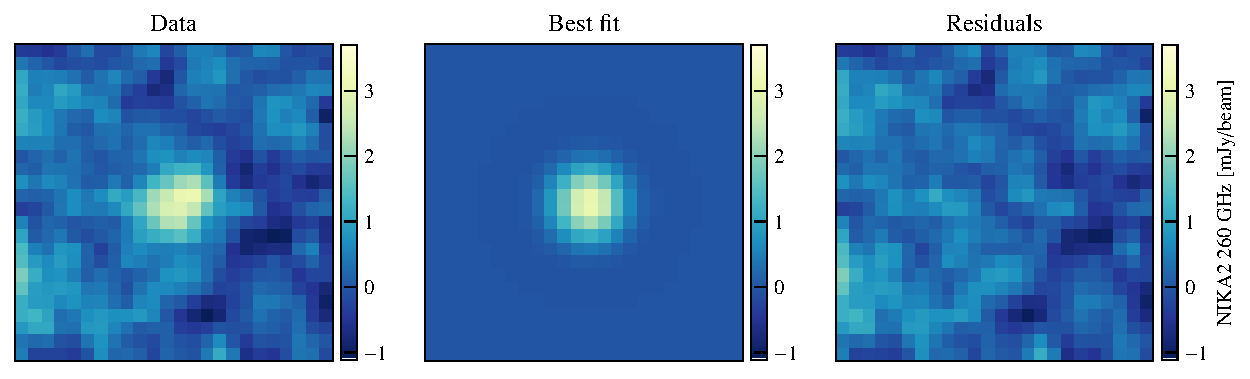
\includegraphics[width=.7\linewidth]{Figures/Chap_decor/4_1mm_fit.pdf}
    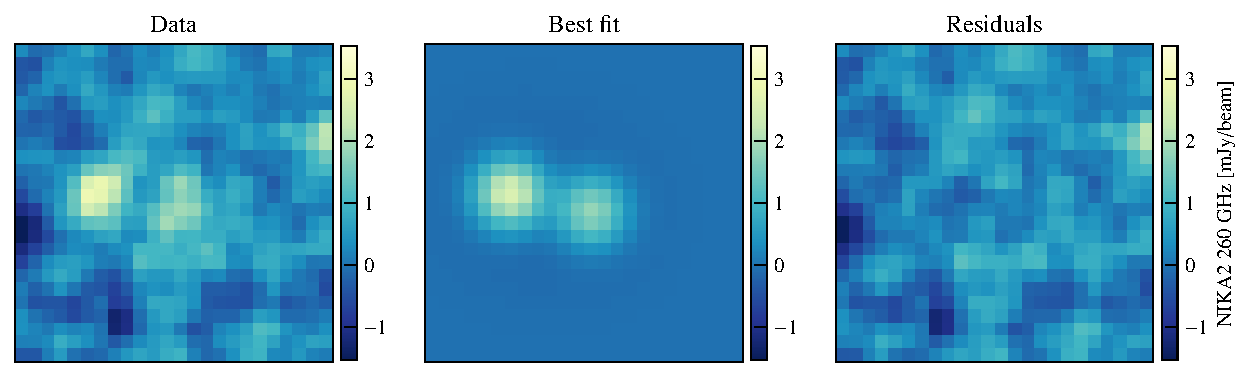
\includegraphics[width=.7\linewidth]{Figures/Chap_decor/2_1mm_fit.pdf}
    \caption{
        Résultats d'un ajustement de source à 260 GHz pour une source simple (\textit{haut}) et pour deux sources proches traitées comme double (\textit{bas}) dans le champ de l'amas \act.
        De gauche à droite, les cartes représentent les données NIKA2 à 260 GHz, le modèle correspondant au meilleur ajustement, et la différence entre les deux cartes.
    }
    \label{fig:pstools_1mm}
\end{figure*}

% ------------------------------------------------------------------------------------- %
\subsection{Ajustement du spectre de chaque source}

Le flux à 260 GHz de chaque source est ensuite combiné avec les trois flux SPIRE, permettant une couverture spectrale allant de 260 à 1200 GHz.
La SED de chaque source est ensuite ajustée sur ces quatre flux, en utilisant un modèle d'émission de corps noir modifié:
\begin{equation}
    F(\nu) = A_0 \left(\frac{\nu}{\nu_0}\right)^\beta B_\nu(T),
    \label{eq:pstools:sed}
\end{equation}
où $B_\nu(T)$ est le spectre d'un corps noir de température $T$, $A_0$ est l'amplitude de la SED à une fréquence de référence $\nu_0 = 500 \; \mathrm{GHz}$, $\beta$ est l'indice spectral de la poussière, et $T$ sa température effective, dégénérée avec le redshift de la source $z$ comme $T = T_\mathrm{dust} / (1+z)$.

L'ajustement de chaque SED est effectué en utilisant un échantillonnage Monte Carlo à chaînes de Markov (MCMC) et la librairie Python \texttt{emcee} \cite{foreman-mackey_emcee_2019}.
Le principe de fonctionnement du MCMC sera présenté au chapitre \ref{chap:panco}.
Nous considérons une fonction de vraisemblance gaussienne.
Lorsque les flux des sources ponctuelles dans les bandes de PACS ne sont pas disponibles, la couverture spectrale est relativement étroite, et ne permet pas de lever la dégénérescence entre les trois paramètres du modèle de corps noir modifié \cite{desert_submillimetre_2008,magnelli_herschel_2012,smith_isothermal_2013}.
Il n'est donc pas possible de laisser ces paramètres complètement libres, avec des \prior\ non-informatifs.
La normalisation de la SED, $A_0$, est donc ajustée linéairement sur les données et fixée pour chaque ajustement.
Un \prior\ sur l'indice spectral de chaque source est imposé par une distribution gaussienne $\beta \sim \N(2, 0.5)$, tel que suggéré par les mesures de SED de grands nombres de galaxies (voir par exemple \cite{magnelli_herschel_2012}).
Enfin, un \prior\ uniforme est utilisé pour la température effective de chaque source, $0 < T < 50 \; \mathrm{K}$.

À chaque étape du MCMC, une correction de couleur est appliquée aux flux mesurés afin de tenir compte de la différence entre le spectre de chaque source et celui de référence utilisé pour l'étalonnage des cartes.
Pour les flux SPIRE, la correction de couleur est interpolée \`a partir de mesures existantes\footnotemark ; pour le flux NIKA2, nous utilisons les corrections décrites dans \cite{perotto_calibration_2020}.
\footnotetext{\url{http://herschel.esac.esa.int/Docs/SPIRE/html/spire_om.html}, \S5.2.7}

À titre illustratif, la partie gauche de la figure \ref{fig:pstools_sed} montre le résultat de cet ajustement pour l'une des sources proches de l'amas \act.
Les flux utilisés pour contraindre le modèle sont représentés par les points bleus, et le modèle de SED résultant par la ligne bleue et les enveloppes d'erreur l'entourant.

\begin{figure}[tp]
    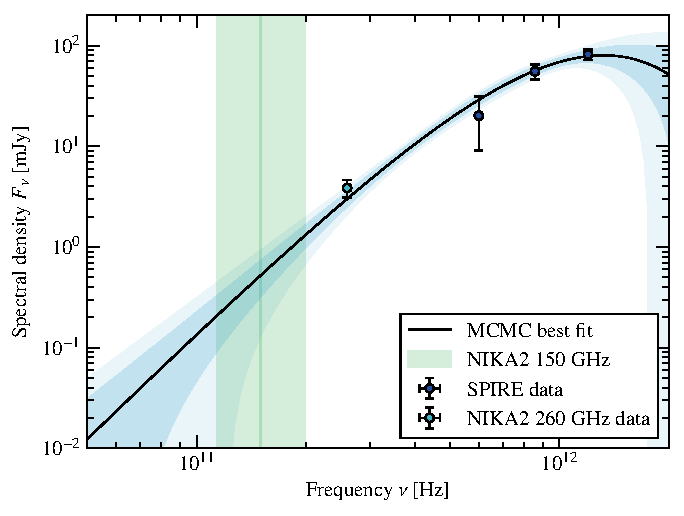
\includegraphics[width=0.48\linewidth]{Figures/Chap_decor/1_SED_no2mm.pdf}
    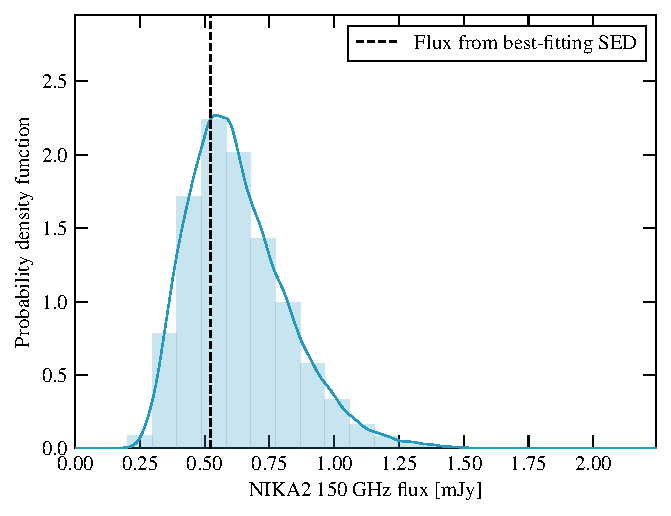
\includegraphics[width=0.48\linewidth]{Figures/Chap_decor/1_2mm_flux_dist.pdf}
    \caption{%
        \textbf{Gauche:} Résultat de l'ajustement de la SED de la source SMG1 dans le champ de l'amas \act, présenté au chapitre \ref{chap:actj0215}.
        Les points bleu foncé représentent des flux SPIRE.
        Les points bleu clair représentent le flux mesuré dans la carte NIKA2 à 260 GHz.
        La ligne bleue montre la SED ajustant le mieux les données, et les enveloppes l'entourant montrent les intervalles de confiance à $1\sigma$ et $2\sigma$.
        La région verte correspond à la bande passante à 150 GHz de NIKA2.
        \textbf{Droite:} Distribution de probabilité du flux de SMG1 dans la bande passante à 150 GHz de NIKA2.
        L'histogramme représente la distribution des flux calculés grâce au MCMC (voir texte).
        La courbe bleue montre la densité de probabilité obtenue en appliquant une estimation par noyaux à cette distribution.
        La ligne verticale noire montre le flux obtenu grâce à la SED ajustant le mieux les données.
        }
        \label{fig:pstools_sed}
\end{figure}

% ------------------------------------------------------------------------------------- %
\subsection{Inférence du flux à 150 GHz}

L'ajustement de SED produit pour chaque source un échantillonnage de la distribution de probabilité dans l'espace des paramètres $(\beta, T)$.
Chaque échantillon de cette distribution est alors utilisé pour calculer une SED grâce à l'équation (\ref{eq:pstools:sed}).
Chacune de ces SED est extrapolée pour calculer une valeur de flux à 150 GHz, et une correction de couleur est appliquée pour en déduire une valeur de flux attendue dans la bande passante de NIKA2.
La distribution de probabilité associée à ce flux est calculée à partir de ces mesures en utilisant une estimation par noyau (KDE pour \textit{Kernel Density Estimation}).
La combinaison de cette mesure avec l'ajustement des sources à 260 GHz nous donne accès, pour chaque source, à une connaissance précise de sa position et de la distribution de probabilité de l'amplitude de sa contamination de l'effet SZ à 150 GHz.
Le résultat de ce calcul est illustré dans la partie droite de la figure \ref{fig:pstools_sed}.

Le produit principal de \texttt{PSTools} est donc la distribution de probabilité du flux de chaque source dans la bande à 150 GHz de NIKA2.
Il existe plusieurs façons d'utiliser cette information pour traiter la contamination due à chaque source.
La plus simple consiste à soustraire un modèle de source à la carte NIKA2, avec un flux donné par le flux le plus probable issu de l'ajustement de SED, correspondant à la valeur maximisant la distribution de probabilités obtenue par \texttt{PSTools}.
Cette approche ne permet toutefois pas de tirer pleinement profit de l'information disponible, par exemple l'incertitude sur ce flux.
Nous verrons au chapitre suivant (section \ref{sec:panco_ps}) que les flux des sources peuvent être traités comme des paramètres de nuisance dans la modélisation de la carte de l'effet SZ d'un amas.
Cette approche permet de propager l'incertitude sur les flux des sources aux propriétés physiques de l'amas en utilisant la distribution de probabilités issue de \texttt{PSTools} comme \prior\ dans l'analyse.

% ===================================================================================== %
\section{Conclusions et perspectives}

Ce chapitre a présenté le traitement des données brutes de NIKA2 pour obtenir des cartes de l'effet SZ.
Nous avons vu en détail le principe de la décorrélation, c'est-à-dire l'extraction du signal astrophysique dans les observations NIKA2 dominées par différentes sources de bruit.
Le calcul de la matrice de covariance du bruit résiduel dans les cartes et du filtrage du signal a également été présenté.
Nous avons également présenté le logiciel \texttt{PSTools}, qui permet d'estimer l'amplitude de la contamination de l'effet SZ par des sources ponctuelles sub-millimétriques en combinant les observations NIKA2 et \textit{Herschel}.
Nous verrons dans le chapitre \ref{chap:panco} comment ces éléments sont inclus dans l'analyse des propriétés physique d'un amas pour tenir compte des effets systématiques qu'ils engendrent.

Comme nous l'avons discuté en \ref{sec:perf_decor}, la décorrélation est un processus imparfait, qui n'est pas en mesure de distinguer parfaitement le bruit du signal d'intérêt.
Sa performance peut se juger sur deux quantités mesurables: le spectre de puissance du bruit résiduel, et le filtrage du signal.
Comme nous le verrons au chapitre suivant, ces quantités servent à la fois de critères pour quantifier la performance de la décorrélation et d'outils pour tenir compte de son imperfection dans l'analyse des cartes NIKA2.
En pratique, le choix d'une méthode est basé sur un compromis entre filtrage et bruit résiduel.
En effet, les méthodes dites agressives, qui permettent d'atteindre un bruit résiduel très faiblement corrélé, sont en général caractérisées par un fort filtrage du signal d'intérêt.
À l'inverse, les méthodes préservant le mieux le signal sont en général moins performantes pour la soustraction du bruit corrélé.
Sur la base de ce compromis, la méthode \textit{common mode one block} est celle retenue pour l'analyse des observations du grand programme SZ de NIKA2.
Elle permet d'obtenir un filtrage relativement faible du signal aux échelles angulaires d'intérêt pour l'étude des amas de galaxies du grand programme SZ, au prix d'un bruit résiduel très corrélé.

Au sein du grand programme SZ de NIKA2, la décorrélation est réalisée à l'aide du \textit{pipeline} de la collaboration NIKA2, fruit d'un effort de la collaboration pour obtenir un outil permettant de passer des données en temps aux cartes du ciel.
J'ai développé un logiciel basé sur ce \textit{pipeline} pour réaliser ce traitement dans le cas des observations du grand programme SZ.
Ce logiciel permet d'interroger la base de données AMI du grand programme SZ, décrite en section \mypageref{sec:nk_ami}, pour obtenir la liste de \textit{scans} associés à un amas, réaliser la décorrélation de ces \textit{scans} et les coadditionner, puis de calculer la matrice de covariance du bruit résiduel et la fonction de transfert de la décorrélation.
Il a été mis à disposition de la collaboration, et est aujourd'hui systématiquement utilisé pour le traitement des données brutes des amas du grand programme SZ.

La décorrélation telle que présentée dans ce chapitre représente donc la procédure standard pour la décorrélation des données NIKA2 du grand programme SZ à l'heure de l'écriture de cette thèse.
L'amélioration de la procédure est toutefois un sujet très actif au sein de la collaboration NIKA2.
Parmi les axes d'amélioration en cours d'étude, de nouvelles méthodes de décorrélation sont en cours de développement et de test.
On notera en particulier le développement de méthodes novatrices, basées sur une décorrélation itérative sans masque.
Dans ces méthodes, à une itération $i$, plutôt que de masquer la région contenant du signal significatif dans la carte de l'itération $i-1$ dans le calcul du mode commun, la carte de l'itération $i-1$, supposée dominée par le signal d'intérêt, est soustraite aux données brutes.
L'intérêt est ici d'éviter de devoir estimer des modes communs sur trop peu d'échantillons.
Pour des sources étendues comme des amas de galaxies, masquer la région dans laquelle du signal est présent peut laisser peu de détecteurs pour l'estimation du mode commun, résultant en une mauvaise estimation du bruit.
Le processus itératif permet alors de converger vers une carte contenant le signal d'intérêt en ayant mieux retiré le bruit.
Ces méthodes ont mené à plusieurs tests au cours de cette thèse, dont les résultats sont encore très préliminaires.
Elles montrent une performance remarquable dans la soustraction du bruit corrélé, mais un filtrage important du signal astrophysique, qui est encore mal compris.
C'est pourquoi \textit{common mode one block} reste la méthode choisie pour les observations d'amas de galaxies avec NIKA2.

Un autre axe en cours de développement, intimement lié avec le développement de nouvelles méthodes, est le calcul de la fonction de transfert de la décorrélation.
La procédure présentée en \ref{sec:transfer_function} se base sur plusieurs hypothèses.
L'une de ces hypothèses a été discutée: nous avons supposé que le filtrage subi par le signal simulé au cours de notre analyse était identique à celui subi par le signal astrophysique d'intérêt.
En réalité, ces deux filtrages ne sont vraisemblablement pas exactement identiques.
La décorrélation de deux jeux de données, contenant le même bruit, mais dont l'un contient environ deux fois plus de signal que l'autre, peut être différente.
En particulier, les régions en périphérie du masque, dans lesquelles on trouve du signal significatif à $\lesssim 3\sigma$ dans l'analyse des données brutes de NIKA2, contiendront du signal plus significatif dans les données contenant le signal simulé.
Il est donc possible que l'estimateur de fonction de transfert présenté en \ref{sec:transfer_function} ne soit pas complètement juste.
Afin de quantifier cet effet, un travail est en cours pour créer des TOI entièrement synthétiques, contenant un bruit corrélé réaliste et du signal astrophysique pour chaque détecteur.
L'objectif est d'appliquer la procédure de décorrélation à ces TOI simulées pour évaluer la différence entre le filtrage réellement subi par un signal simulé, et l'estimateur de fonction de transfert présenté précédemment. \\
Une autre hypothèse implicite dans l'équation (\ref{eq:transfer_function}) est celle de l'isotropie du filtrage, c'est-à-dire de la symétrie circulaire du rapport entre les transformées de Fourier des cartes d'entrée et de sortie.
Cette hypothèse est justifiée par la stratégie de \textit{scan} du grand programme SZ de NIKA2, discutée en \ref{sec:map_coadd}, qui permet une couverture très isotrope de la région cartographiée en utilisant des \textit{scans} à différents angles.
Cependant, certaines directions peuvent rester privilégiées dans le filtrage, notamment les directions des \textit{scans}.
Une étude est donc en cours pour quantifier l'écart à la symétrie circulaire du filtrage subi par le signal d'intérêt lors de la décorrélation.
Les résultats en sont très prometteurs, montrant l'intérêt de l'utilisation de fonctions de transfert à deux dimensions pour les analyses du grand programme SZ \cite{munoz_echevarria_multi-probe_2021}.

La décorrélation reste donc un sujet d'étude actif, et les prochaines années permettront des avancées pour maximiser la qualité des cartes de l'effet SZ construites grâce aux observations NIKA2.
